\documentclass[twocolumn, 10pt,a4j]{jsarticle}
\usepackage{amsmath}
\usepackage{here}
\usepackage[dvipdfmx]{graphicx}
\usepackage{url}
% プリアンブル
\title{\vspace{-2.5cm}ロボットの基礎}
\author{1610581 堀田 大地}
\date{2018/11/21}
\begin{document}
\maketitle{}
\section{目的}
% 目的
  ロボットを用いて各種制御実験を行い,ロボットの各種制御法,運動学,動力学,冗長性について理解する.

\section{実験課題}
% 実験課題
  \subsection{課題 1.}
    目標値が時不変の場合についてPD制御,重力補償つきPD制御,フィードバック線形化制御をゲインを小,中,大で実行した結果を考察する. 結果を図1 $\to$ 18に示す.
    \begin{enumerate}
      \item 制御方法,ゲインと制御結果の関係についての考察.
        PD制御,重力補償つきPD制御,フィードバック線形化制御の全ての制御はゲインが大きくなるほど最終姿勢は定性的に評価すると良くなっていた.
        さらに,時間応答でも,振動が少なくなっていく傾向が見られた. 本実験では,PD制御,重力補償つきPD制御,フィードバック線形化制御の全ての制御はゲインが大きくなるほど
        目標位置の近づけるようになっていたことを確認できた.

      \item 「良好な結果が得られた」と言える制御方法とゲインの組み合わせをあげ定量的に評価.
        題意を満たす条件はフィードバック線形化かつゲインが大きいときであった. 同じフィードバック線形化のゲインのパラメータごとの最終的なtau1,2を表1に示す. 表1より,この条件が良いことが定量的に評価できる.
    \end{enumerate}


    %%%%%%%%%%%%%%%%%%%%%%%%%%%%%%%%%%%%%%%%%%%%%%%%%%%%%%%%%%%%%%%%%%%%%%%%%%%%%%%%%%%%%%%%%%%%%%%%%%%
    \begin{figure}[H]
      % 図1
      \begin{center}
        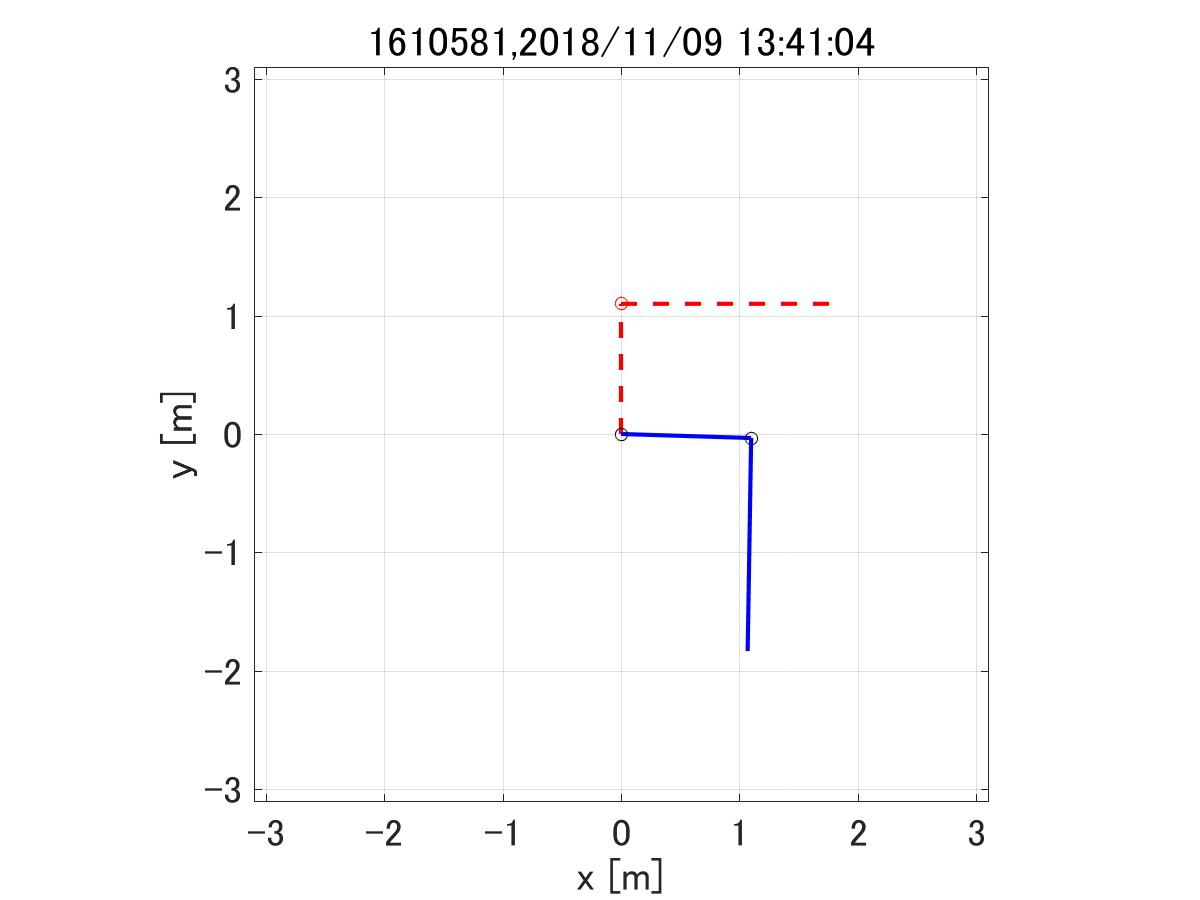
\includegraphics[width=7cm]{../img/img/kansetu_PD_zifuhen_small_no_model_gosa_saisyu_sisei.jpg}
        \caption{時不変のときPD制御を用いてゲインを小,モデル誤差なしと設定したときの最終姿勢.}
      \end{center}
    \end{figure}

    \begin{figure}[H]
      % 図2
      \begin{center}
        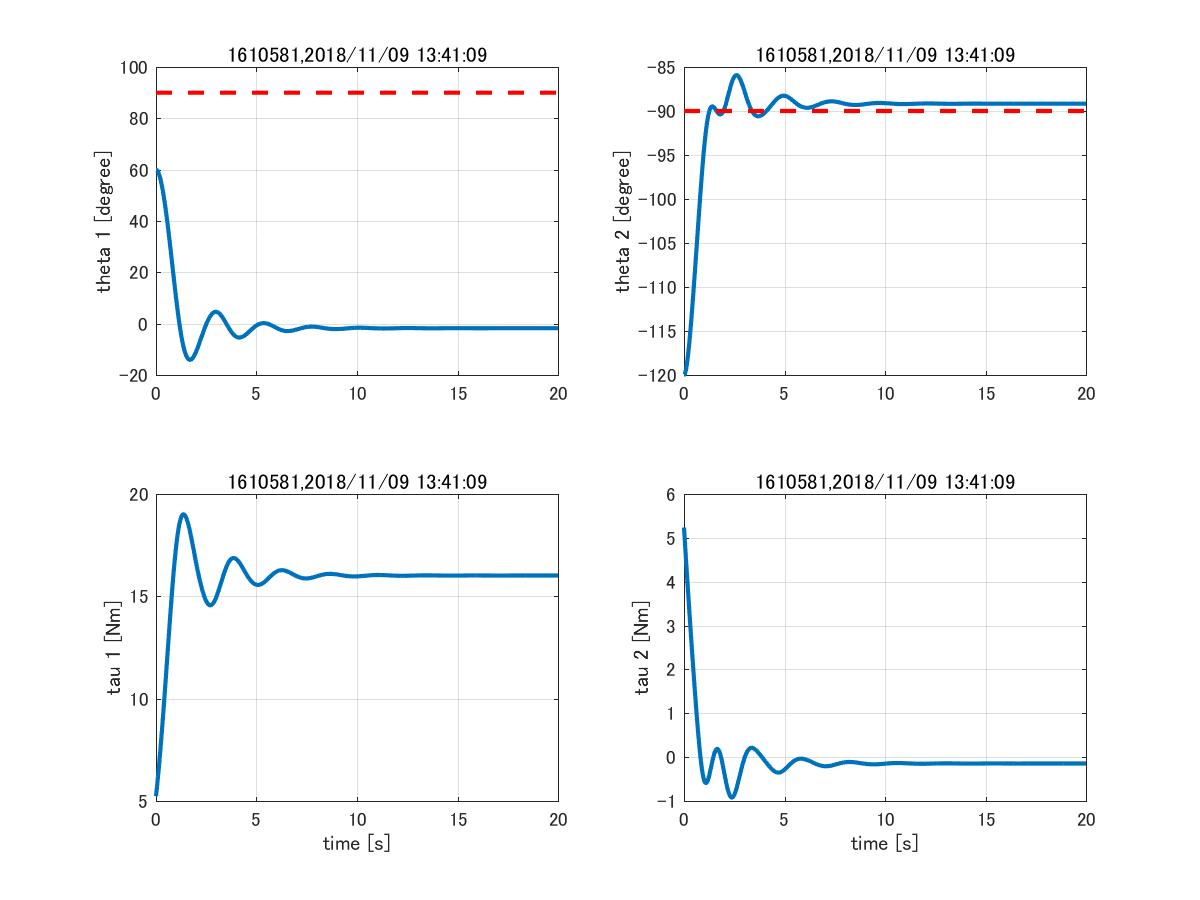
\includegraphics[width=7cm]{../img/img/kansetu_PD_zifuhen_small_no_model_gosa_zikan_outo.jpg}
        \caption{時不変のときPD制御を用いてゲインを小,モデル誤差なしと設定したときの時間応答.}
      \end{center}
    \end{figure}
    %%%%%%%%%%%%%%%%%%%%%%%%%%%%%%%%%%%%%%%%%%%%%%%%%%%%%%%%%%%%%%%%%%%%%%%%%%%%%%%%%%%%%%%%%%%%%%%%%%%
    \begin{figure}[H]
      % 図3
      \begin{center}
        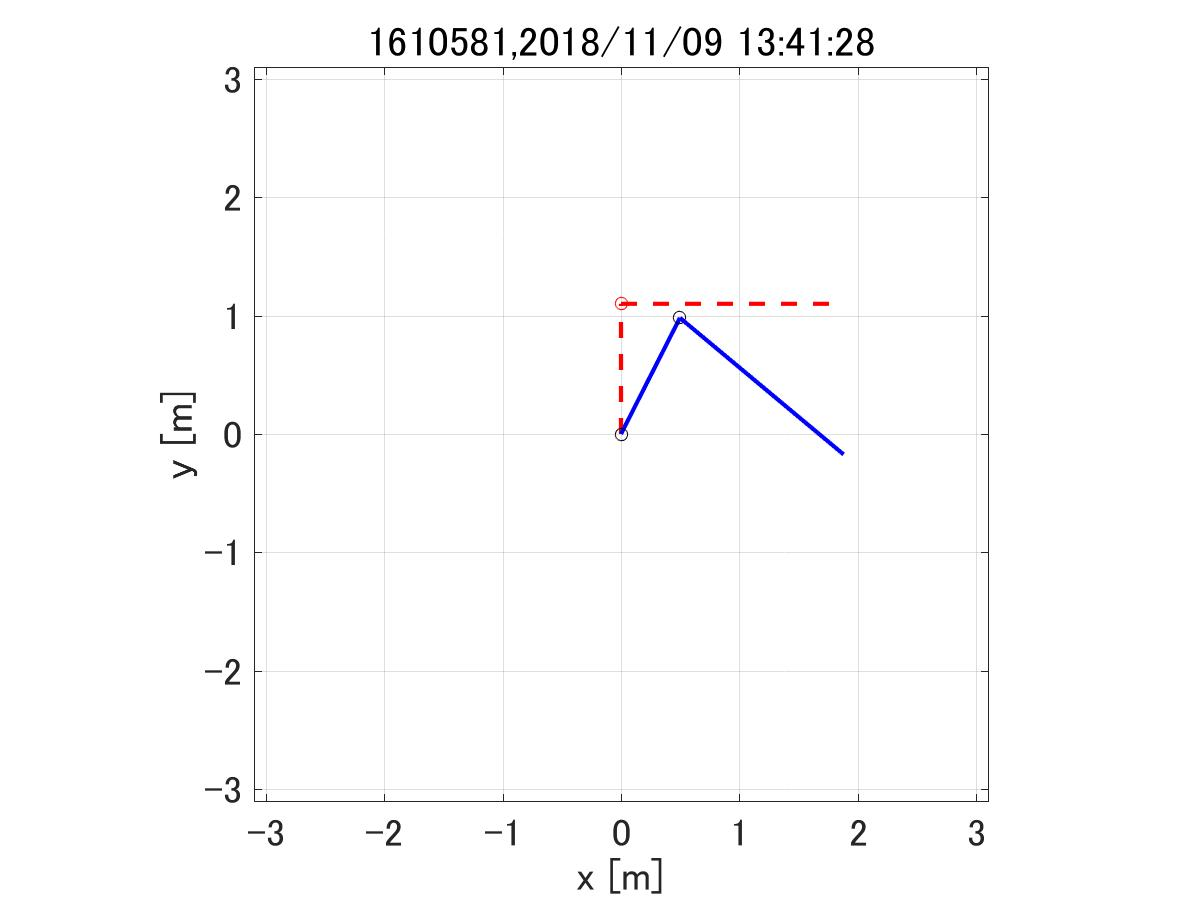
\includegraphics[width=7cm]{../img/img/kansetu_PD_zifuhen_chu_no_model_gosa_saisyu_sisei.jpg}
        \caption{時不変のときPD制御を用いてゲインを中,モデル誤差なしと設定したときの最終姿勢.}
      \end{center}
    \end{figure}

    \begin{figure}[H]
      % 図4
      \begin{center}
        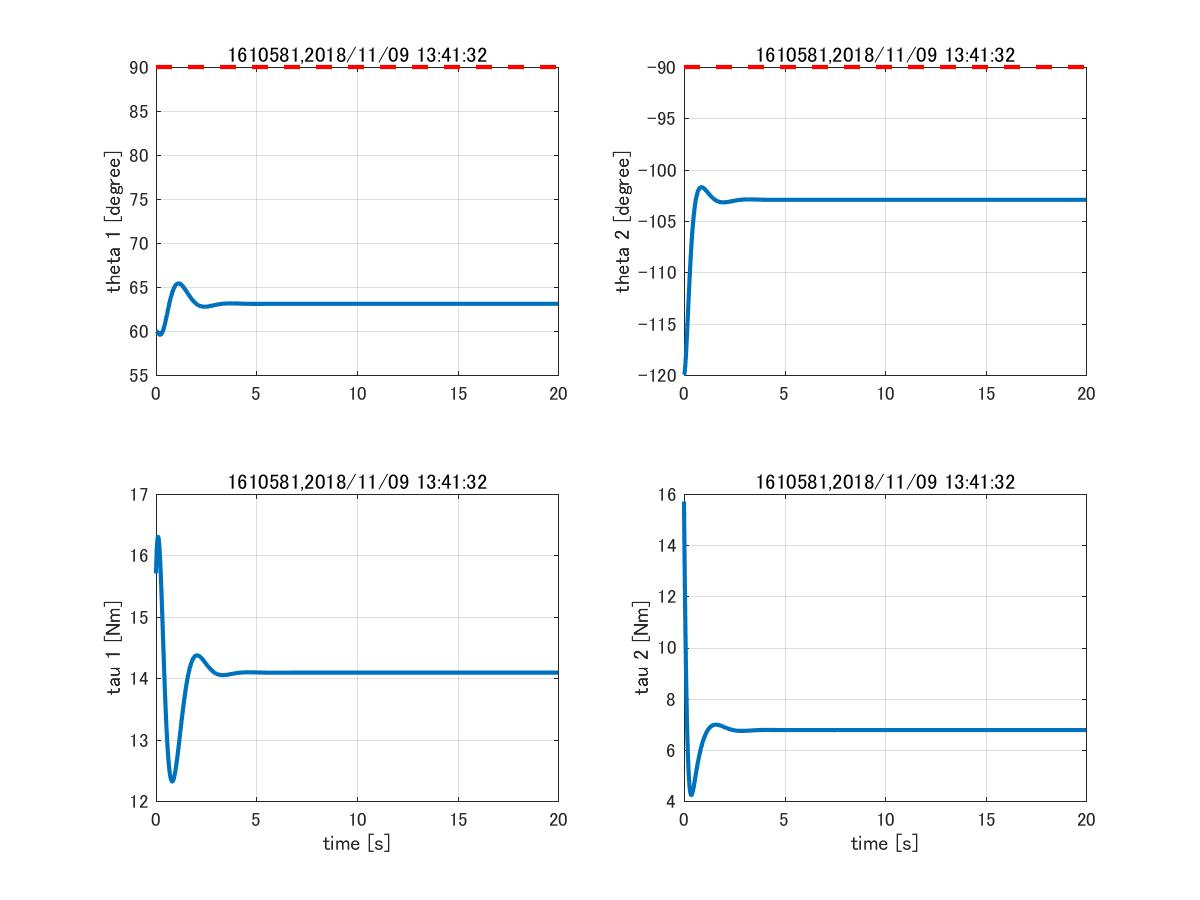
\includegraphics[width=7cm]{../img/img/kansetu_PD_zifuhen_chu_no_model_gosa_zikan_auto.jpg}
        \caption{時不変のときPD制御を用いてゲインを中,モデル誤差なしと設定したときの時間応答.}
      \end{center}
    \end{figure}
    %%%%%%%%%%%%%%%%%%%%%%%%%%%%%%%%%%%%%%%%%%%%%%%%%%%%%%%%%%%%%%%%%%%%%%%%%%%%%%%%%%%%%%%%%%%%%%%%%%%
    \begin{figure}[H]
      % 図5
      \begin{center}
        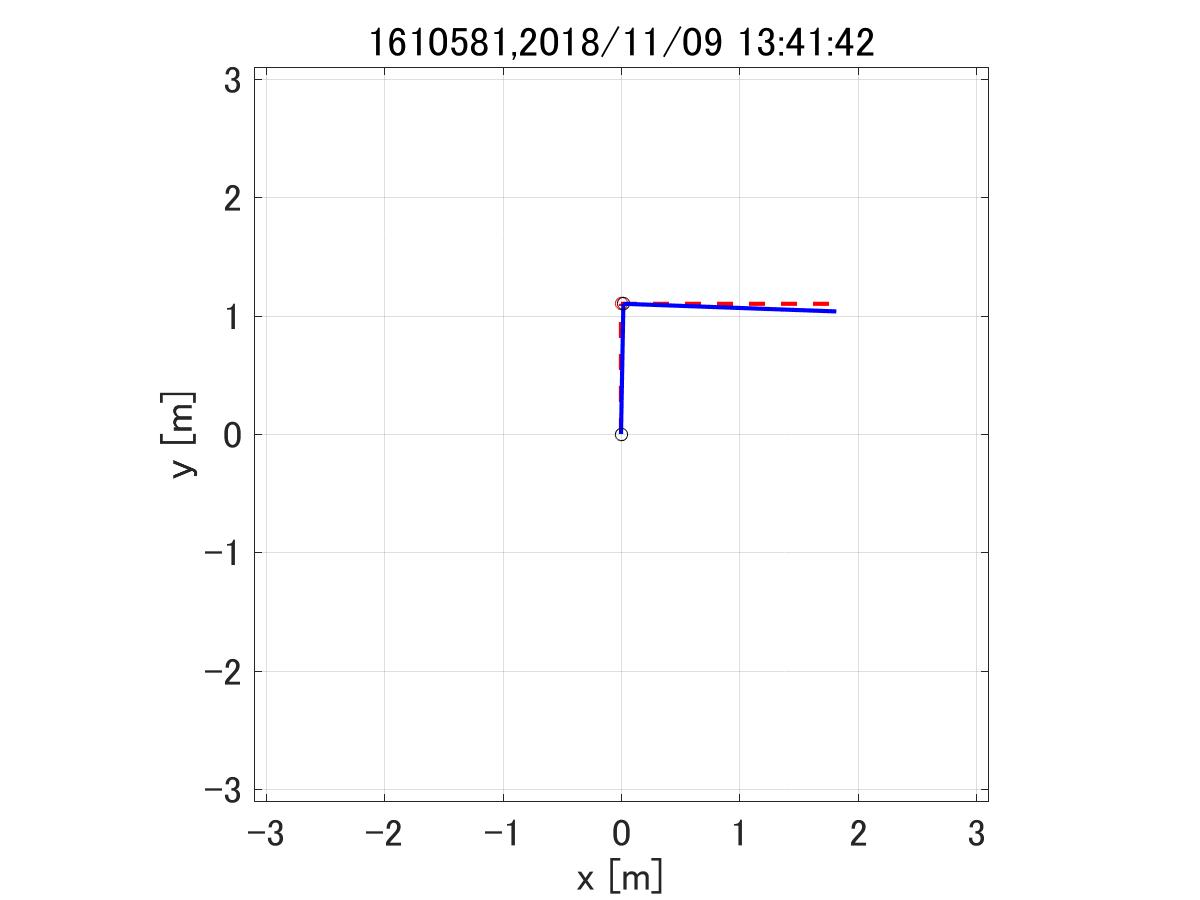
\includegraphics[width=7cm]{../img/img/kansetu_PD_zifuhen_large_no_model_gosa_saisyu_sisei.jpg}
        \caption{時不変のときPD制御を用いてゲインを大,モデル誤差なしと設定したときの最終姿勢.}
      \end{center}
    \end{figure}

    \begin{figure}[H]
      % 図6
      \begin{center}
        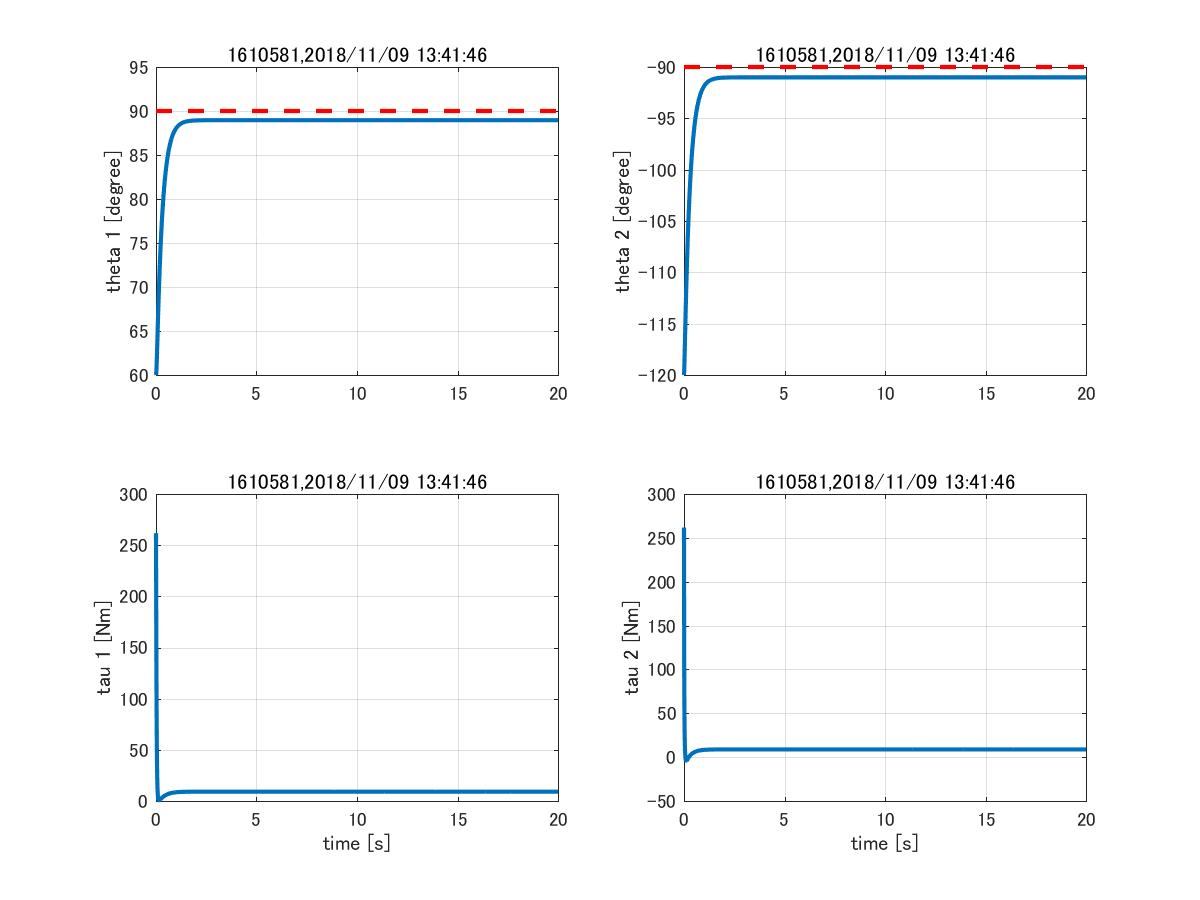
\includegraphics[width=7cm]{../img/img/kansetu_PD_zifuhen_large_no_model_gosa_zikan_auto.jpg}
        \caption{時不変のときPD制御を用いてゲインを大,モデル誤差なしと設定したときの時間応答.}
      \end{center}
    \end{figure}
    %%%%%%%%%%%%%%%%%%%%%%%%%%%%%%%%%%%%%%%%%%%%%%%%%%%%%%%%%%%%%%%%%%%%%%%%%%%%%%%%%%%%%%%%%%%%%%%%%%%
    \begin{figure}[H]
      % 図5
      \begin{center}
        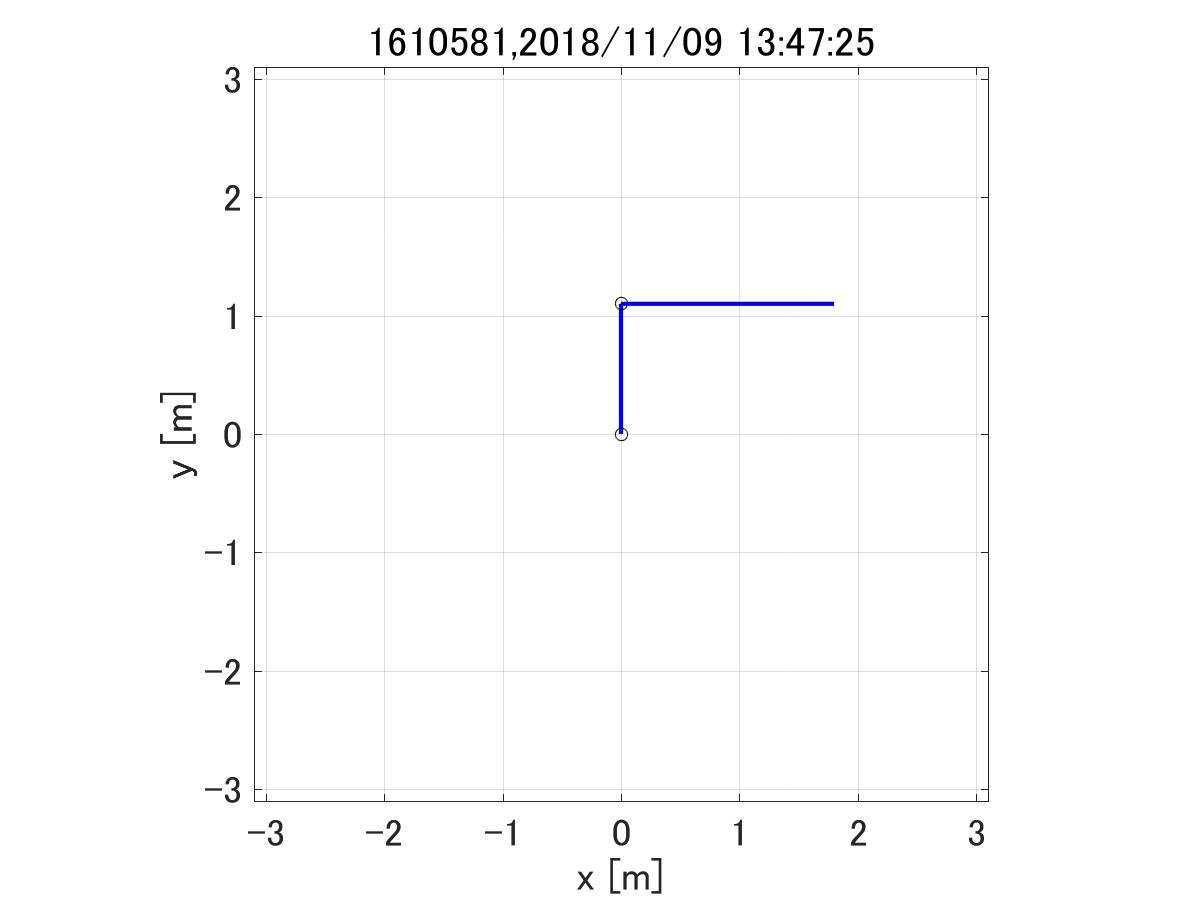
\includegraphics[width=7cm]{../img/img/kansetu_juryoku_hosyou_PD_zifuhen_small_no_model_gosa_saisyu_sisei.jpg}
        \caption{時不変のとき重力補償つきPD制御を用いてゲインを小,モデル誤差なしと設定したときの最終姿勢.}
      \end{center}
    \end{figure}

    \begin{figure}[H]
      % 図6
      \begin{center}
        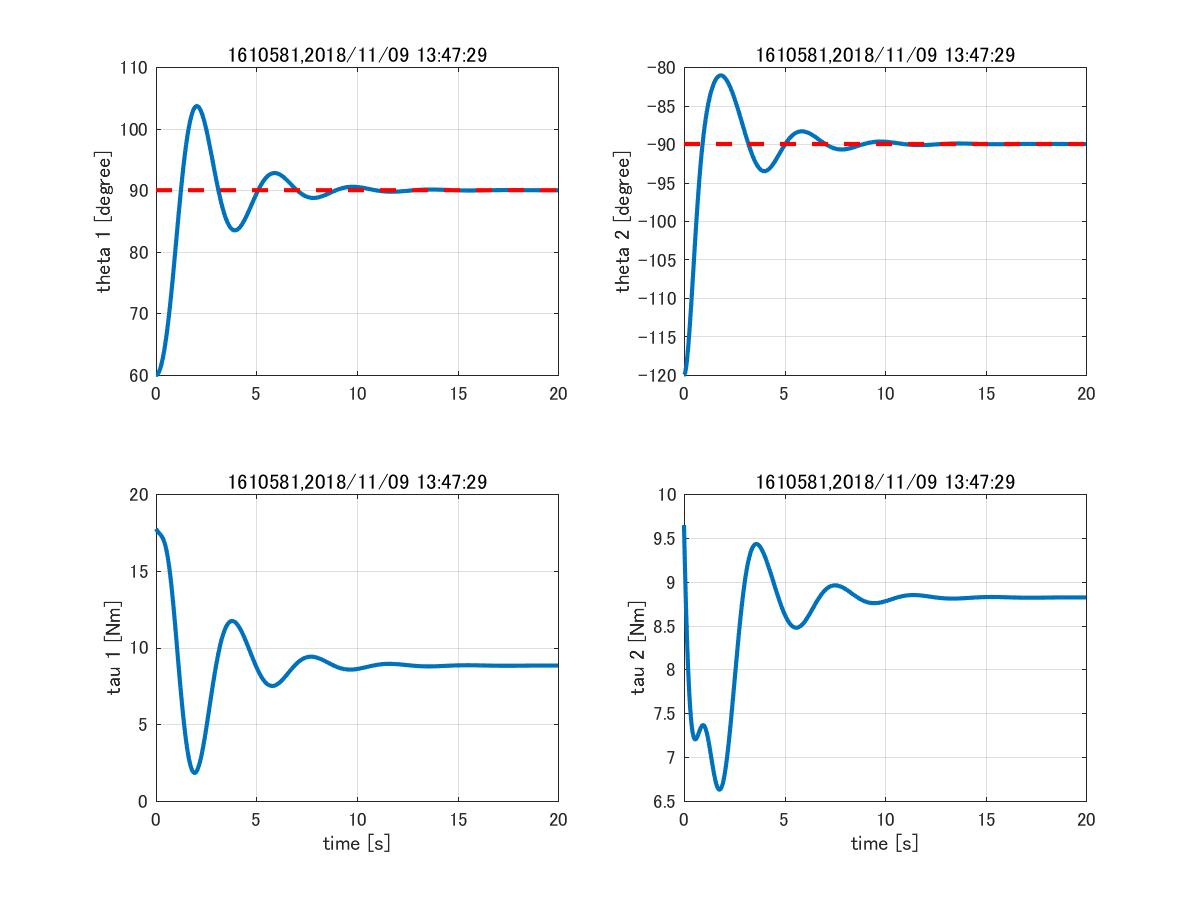
\includegraphics[width=7cm]{../img/img/kansetu_juryoku_hosyou_PD_zifuhen_small_no_model_gosa_zikan_auto.jpg}
        \caption{時不変のとき重力補償つきPD制御を用いてゲインを小,モデル誤差なしと設定したときの時間応答.}
      \end{center}
    \end{figure}
    %%%%%%%%%%%%%%%%%%%%%%%%%%%%%%%%%%%%%%%%%%%%%%%%%%%%%%%%%%%%%%%%%%%%%%%%%%%%%%%%%%%%%%%%%%%%%%%%%%%
    \begin{figure}[H]
      % 図5
      \begin{center}
        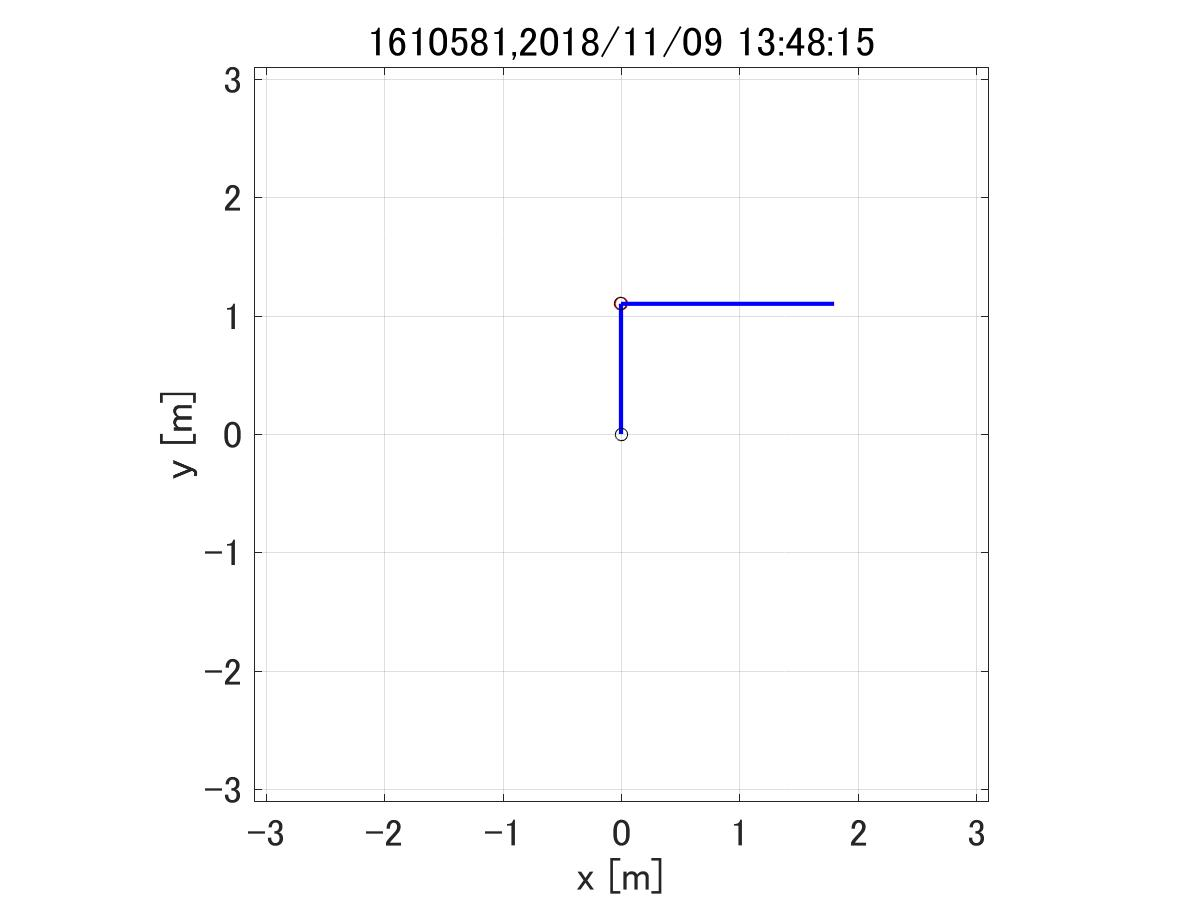
\includegraphics[width=7cm]{../img/img/kansetu_juryoku_hosyou_PD_zifuhen_chu_no_model_gosa_saisyu_sisei.jpg}
        \caption{時不変のとき重力補償つきPD制御を用いてゲインを中,モデル誤差なしと設定したときの最終姿勢.}
      \end{center}
    \end{figure}

    \begin{figure}[H]
      % 図6
      \begin{center}
        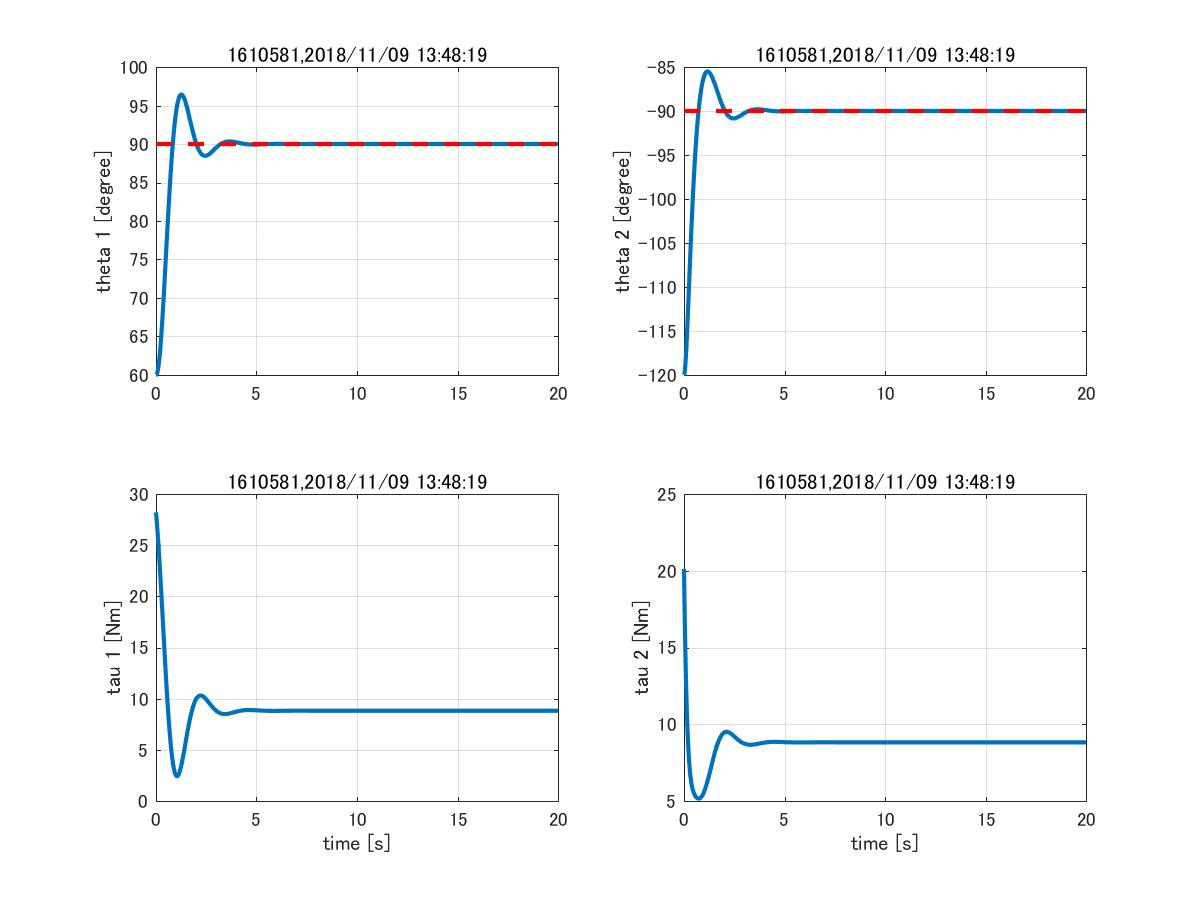
\includegraphics[width=7cm]{../img/img/kansetu_juryoku_hosyou_PD_zifuhen_chu_no_model_gosa_zikan_auto.jpg}
        \caption{時不変のとき重力補償つきPD制御を用いてゲインを中,モデル誤差なしと設定したときの時間応答.}
      \end{center}
    \end{figure}
    %%%%%%%%%%%%%%%%%%%%%%%%%%%%%%%%%%%%%%%%%%%%%%%%%%%%%%%%%%%%%%%%%%%%%%%%%%%%%%%%%%%%%%%%%%%%%%%%%%%
    \begin{figure}[H]
      % 図5
      \begin{center}
        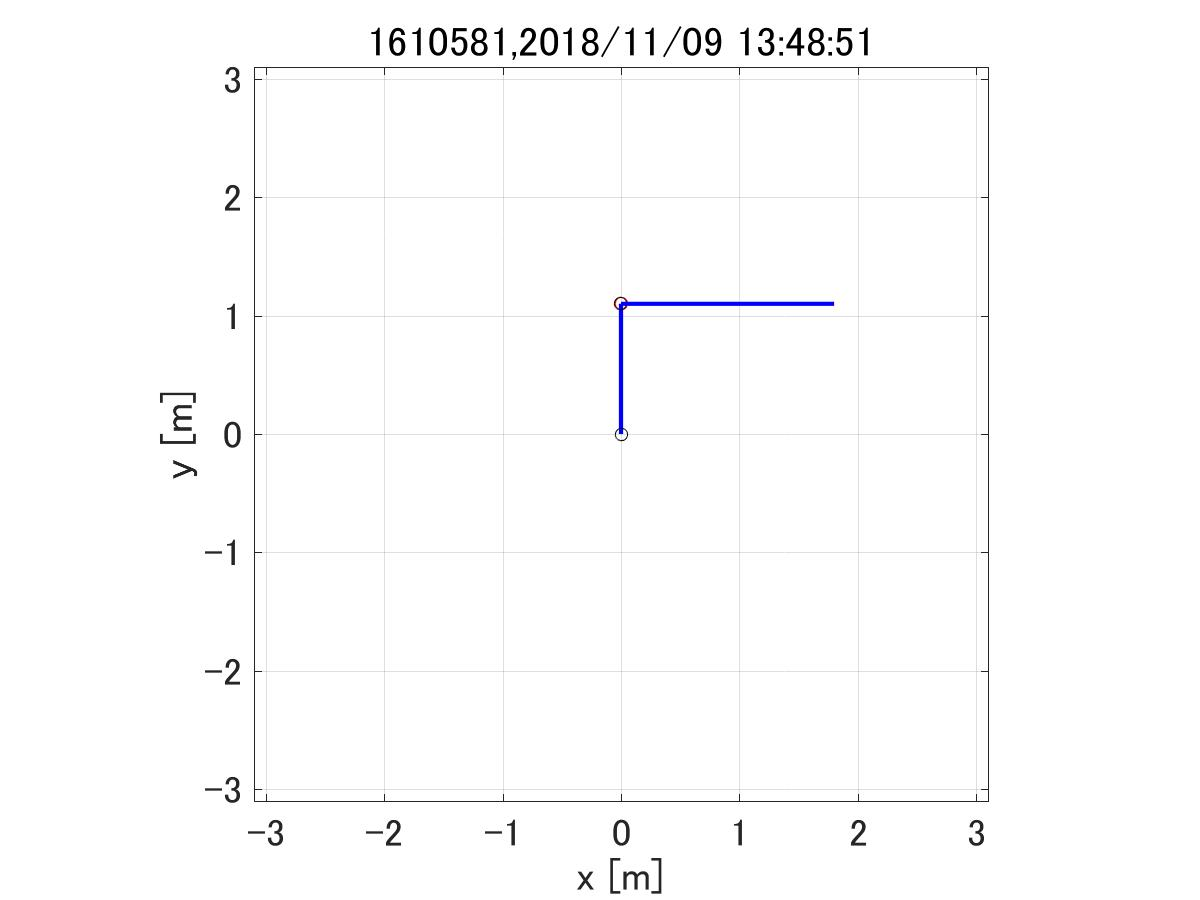
\includegraphics[width=7cm]{../img/img/kansetu_juryoku_hosyou_PD_zifuhen_large_no_model_gosa_saisyu_sisei.jpg}
        \caption{時不変のとき重力補償つきPD制御を用いてゲインを大,モデル誤差なしと設定したときの最終姿勢.}
      \end{center}
    \end{figure}

    \begin{figure}[H]
      % 図6
      \begin{center}
        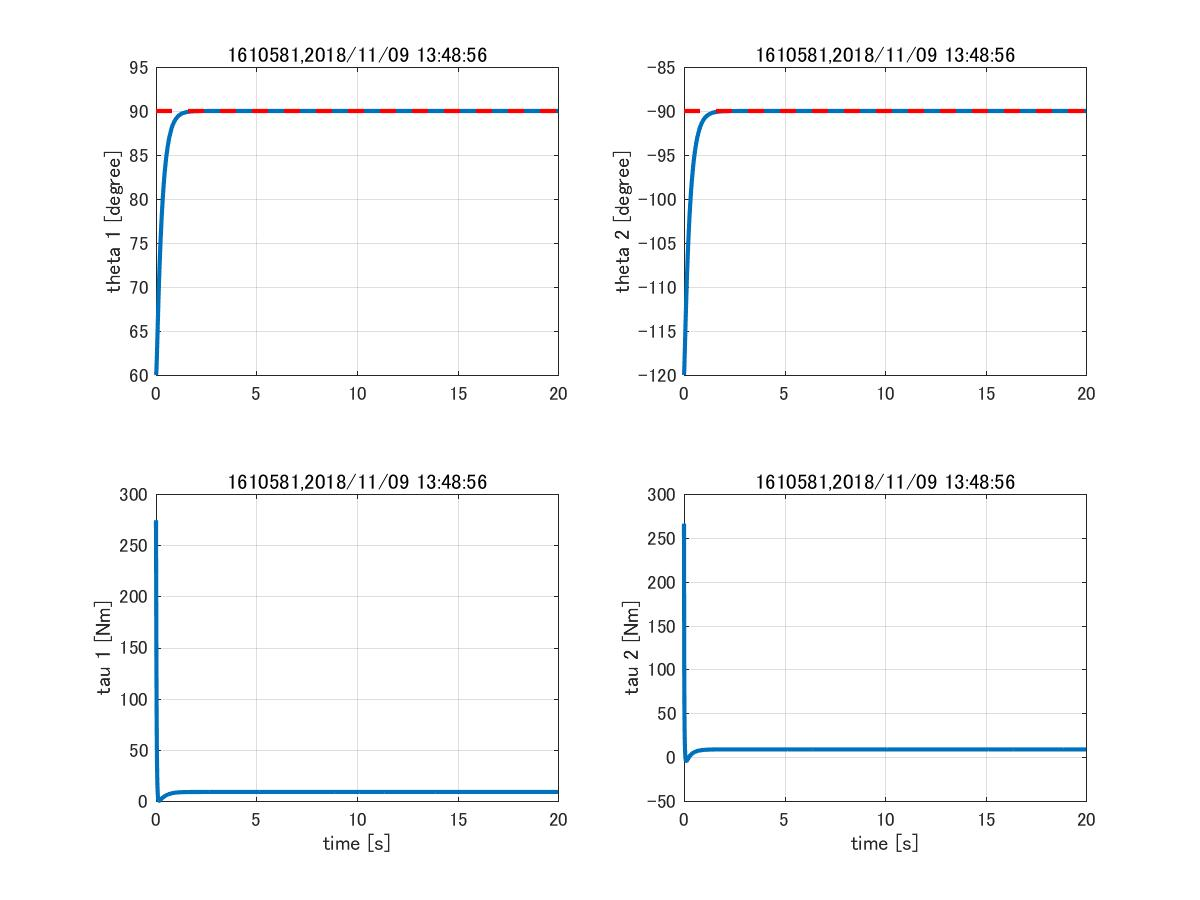
\includegraphics[width=7cm]{../img/img/kansetu_juryoku_hosyou_PD_zifuhen_large_no_model_gosa_zikan_auto.jpg}
        \caption{時不変のとき重力補償つきPD制御を用いてゲインを大,モデル誤差なしと設定したときの時間応答.}
      \end{center}
    \end{figure}
    %%%%%%%%%%%%%%%%%%%%%%%%%%%%%%%%%%%%%%%%%%%%%%%%%%%%%%%%%%%%%%%%%%%%%%%%%%%%%%%%%%%%%%%%%%%%%%%%%%%
    \begin{figure}[H]
      % 図5
      \begin{center}
        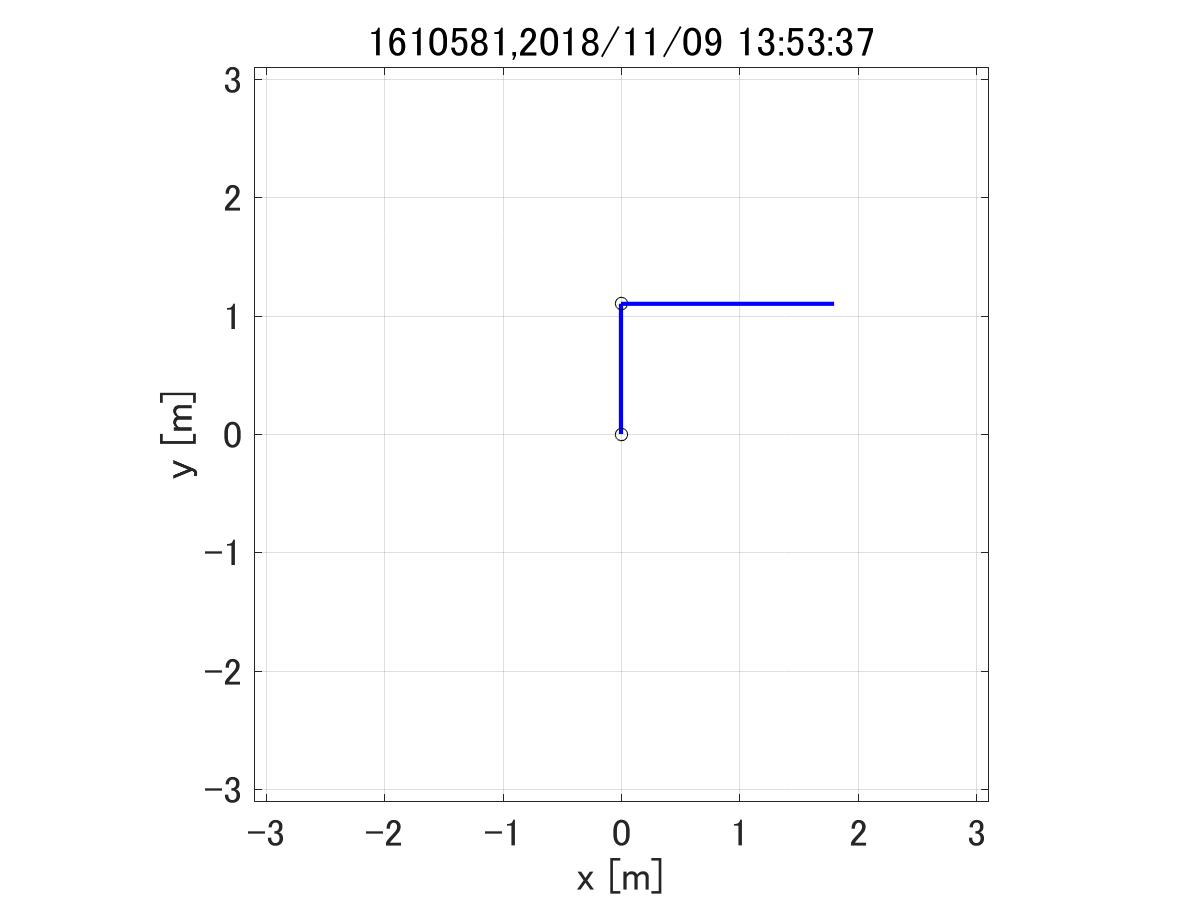
\includegraphics[width=7cm]{../img/img/kansetu_FB_zifuhen_small_no_model_gosa_saisyu_sisei.jpg}
        \caption{時不変のときフィードバック線形化制御を用いてゲインを小,モデル誤差なしと設定したときの最終姿勢.}
      \end{center}
    \end{figure}

    \begin{figure}[H]
      % 図6
      \begin{center}
        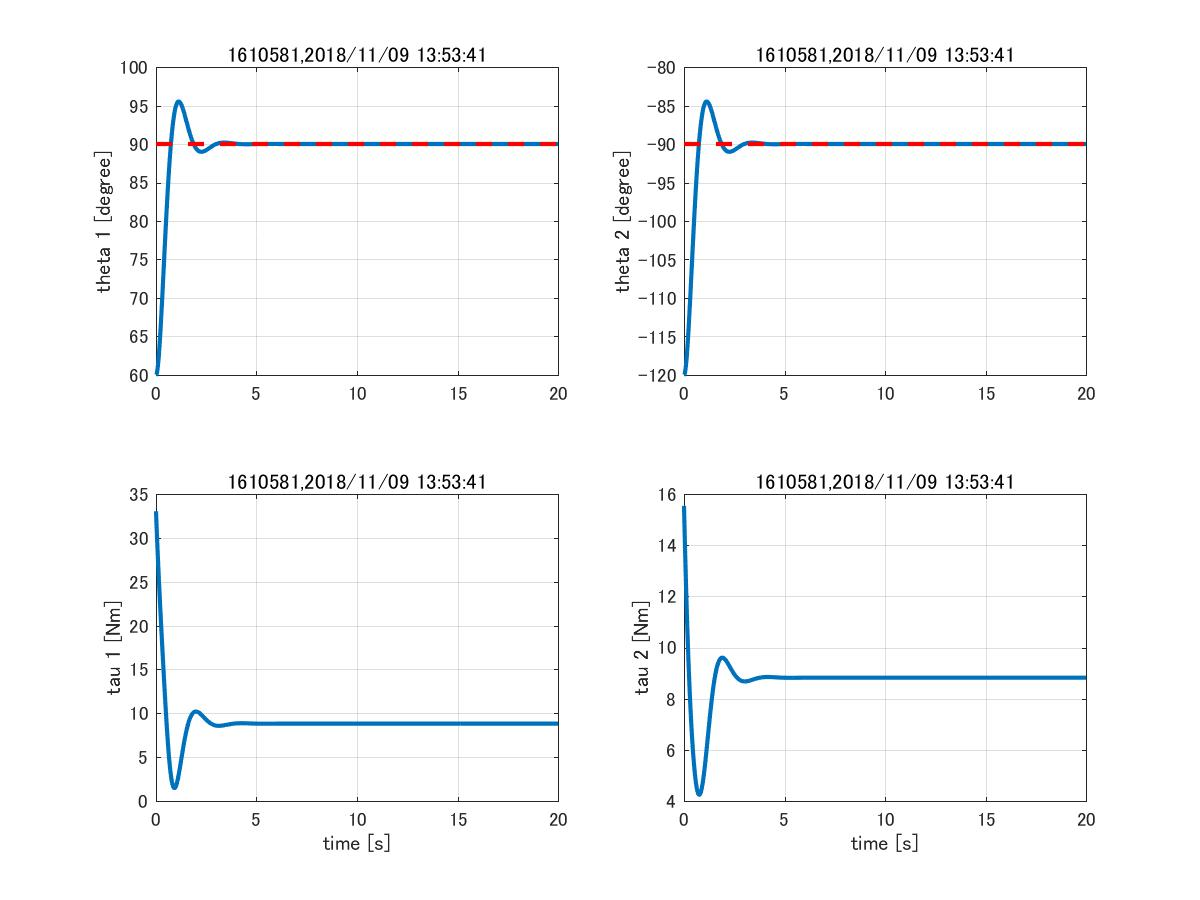
\includegraphics[width=7cm]{../img/img/kansetu_FB_zifuhen_small_no_model_gosa_zikan_auto.jpg}
        \caption{時不変のときフィードバック線形化制御を用いてゲインを小,モデル誤差なしと設定したときの時間応答.}
      \end{center}
    \end{figure}
    %%%%%%%%%%%%%%%%%%%%%%%%%%%%%%%%%%%%%%%%%%%%%%%%%%%%%%%%%%%%%%%%%%%%%%%%%%%%%%%%%%%%%%%%%%%%%%%%%%%
    \begin{figure}[H]
      % 図5
      \begin{center}
        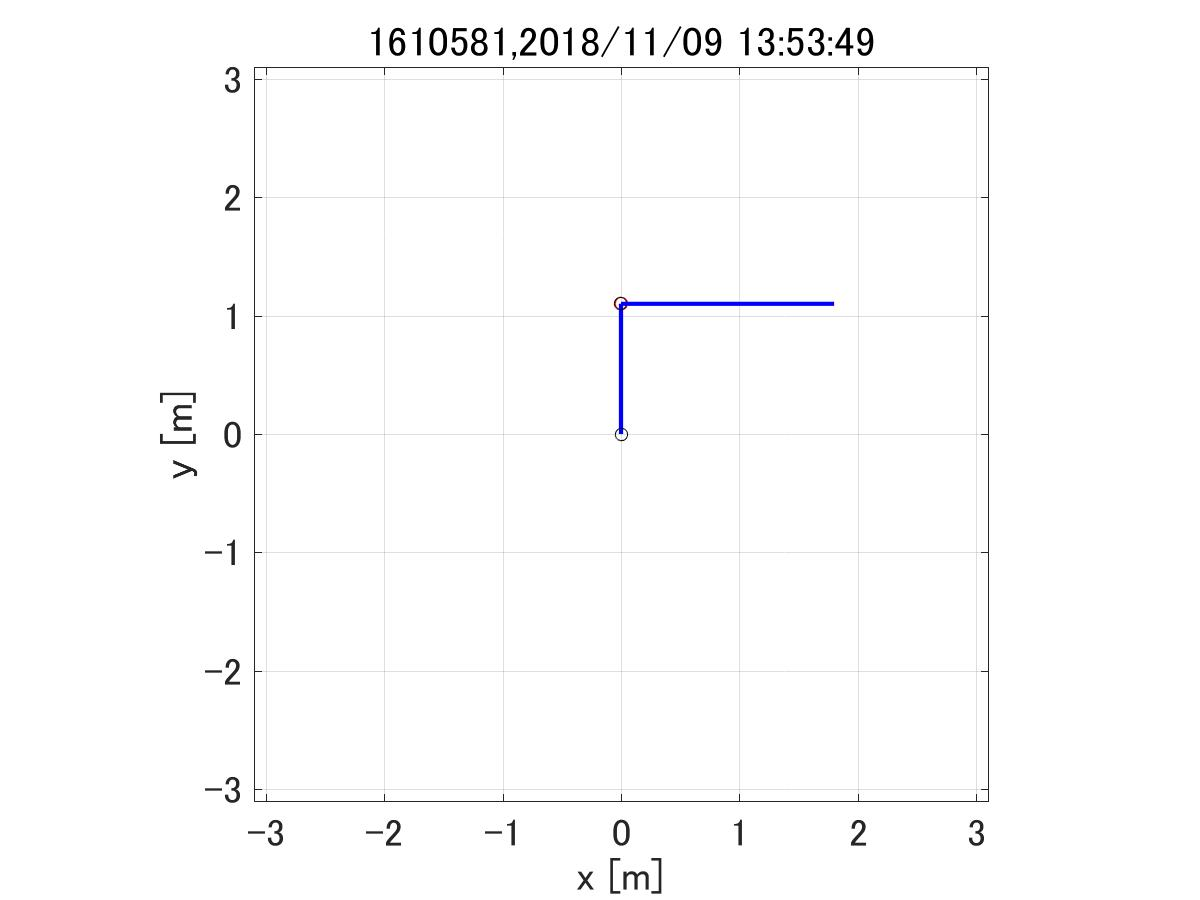
\includegraphics[width=7cm]{../img/img/kansetu_FB_zifuhen_chu_no_model_gosa_saisyu_sisei.jpg}
        \caption{時不変のときフィードバック線形化制御を用いてゲインを中,モデル誤差なしと設定したときの最終姿勢.}
      \end{center}
    \end{figure}

    \begin{figure}[H]
      % 図6
      \begin{center}
        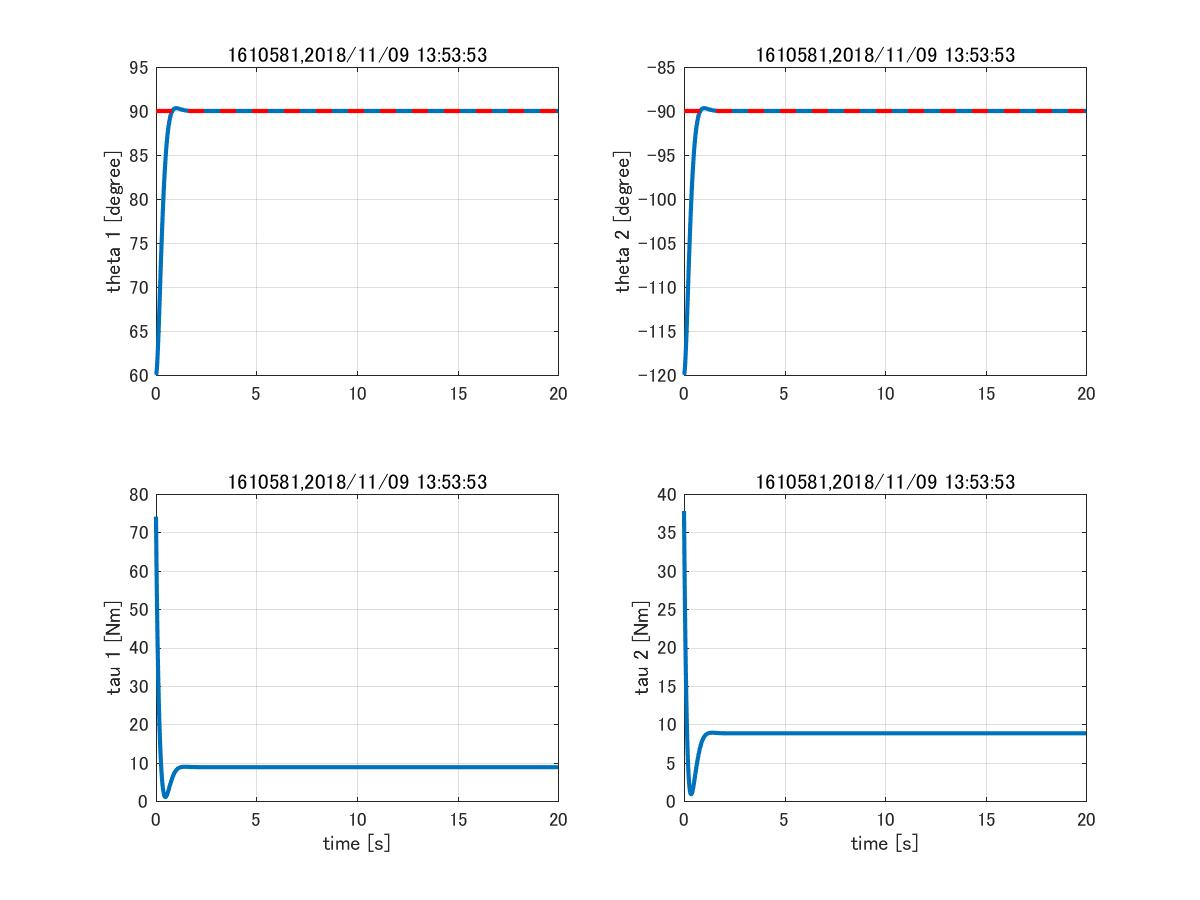
\includegraphics[width=7cm]{../img/img/kansetu_FB_zifuhen_chu_no_model_gosa_zikan_auto.jpg}
        \caption{時不変のときフィードバック線形化制御を用いてゲインを中,モデル誤差なしと設定したときの時間応答.}
      \end{center}
    \end{figure}
    %%%%%%%%%%%%%%%%%%%%%%%%%%%%%%%%%%%%%%%%%%%%%%%%%%%%%%%%%%%%%%%%%%%%%%%%%%%%%%%%%%%%%%%%%%%%%%%%%%%
    \begin{figure}[H]
      % 図5
      \begin{center}
        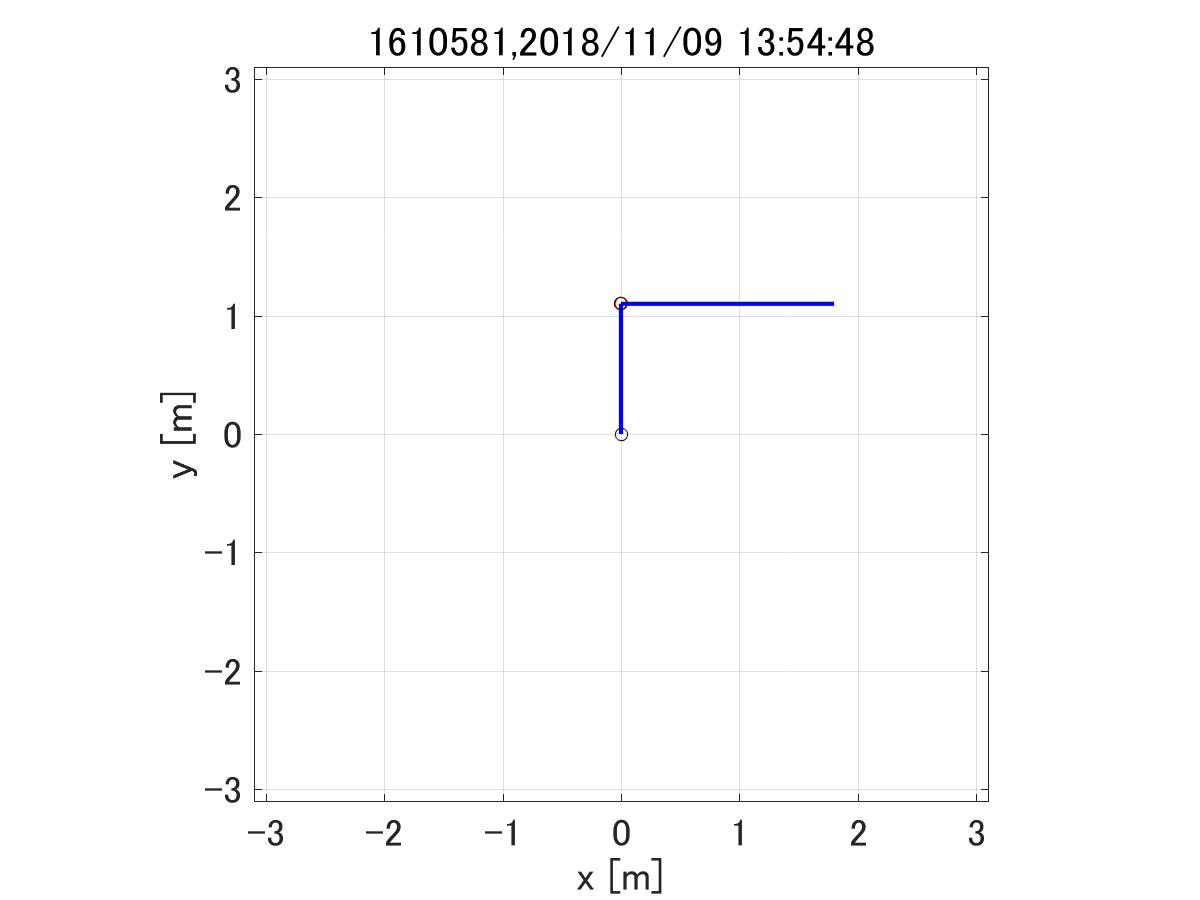
\includegraphics[width=7cm]{../img/img/kansetu_FB_zifuhen_large_no_model_gosa_saisyu_sisei.jpg}
        \caption{時不変のときフィードバック線形化制御を用いてゲインを大,モデル誤差なしと設定したときの最終姿勢.}
      \end{center}
    \end{figure}

    \begin{figure}[H]
      % 図6
      \begin{center}
        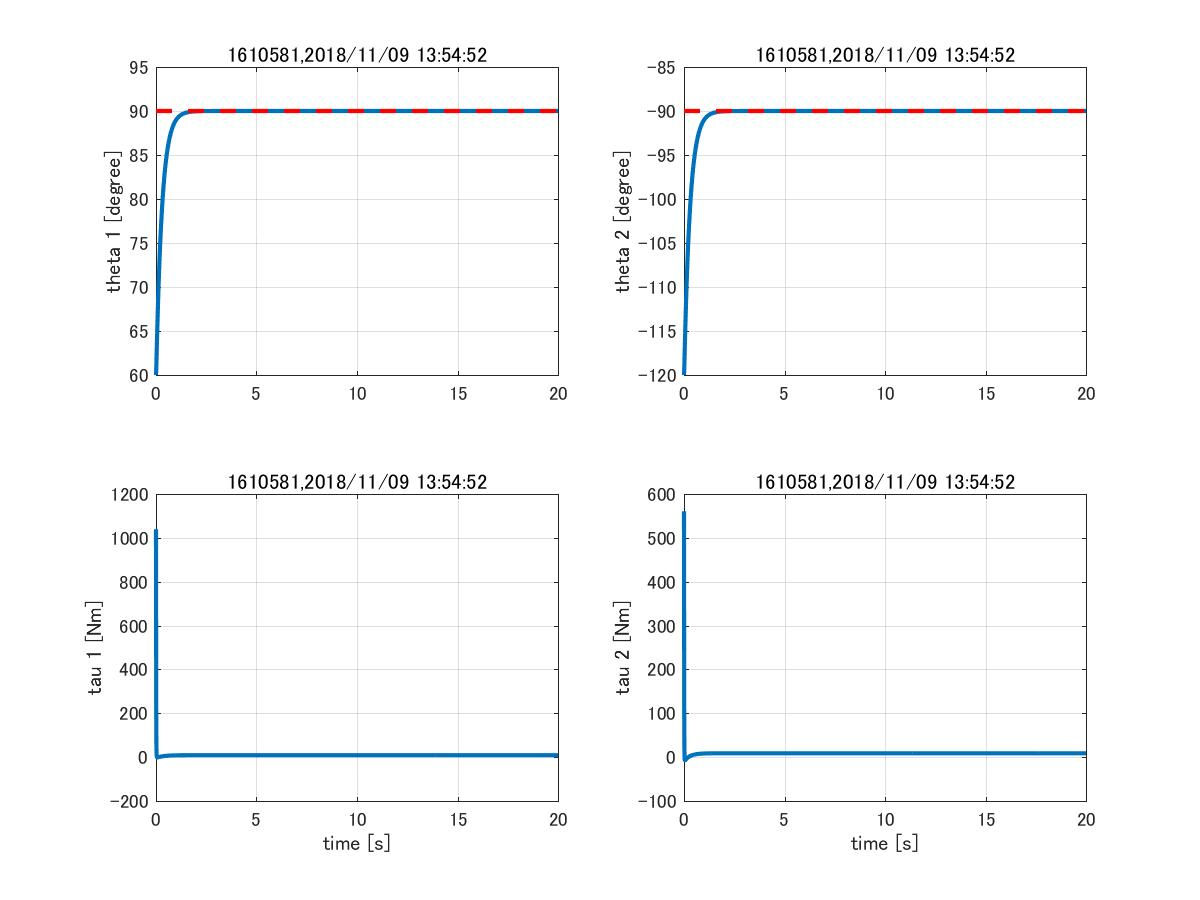
\includegraphics[width=7cm]{../img/img/kansetu_FB_zifuhen_large_no_model_gosa_zikan_auto.jpg}
        \caption{時不変のときフィードバック線形化制御を用いてゲインを大,モデル誤差なしと設定したときの時間応答.}        
      \end{center}
    \end{figure}

    \begin{table}[H]
      \begin{center}
        \caption{フィードバック線形化制御におけて,ゲインパラメータの設定でのTauの値. Tauの値は小さいほど良いと評価する.}
        \begin{tabular}{llll}
        ゲインの値 & 小 & 中  & 大 \\ \hline
        Tau1[Nm] & 8 & 10 & 0 \\
        Tau2[Nm] & 9 & 8  & 0
        \end{tabular}
      \end{center}
    \end{table}

  \subsection{課題 2.}
    % 課題2
    目標値が時変の場合についてPD制御,重力補償つきPD制御,フィードバック線形化制御をゲインを小,中,大で実行した結果を考察する. 結果を図19 $\to$ 36に示す.
    \begin{enumerate}
      \item 制御方法,ゲインと制御結果の関係についての考察.
        PD制御,重力補償つきPD制御,フィードバック線形化制御の全ての制御はゲインが大きくなるほど最終姿勢は定性的に評価すると良くなっていた.
        さらに,時間応答のtauでも,振動が少なくなっていく傾向が見られた. 本実験では,PD制御,重力補償つきPD制御,フィードバック線形化制御の全ての制御はゲインが大きくなるほど
        目標位置の近づけるようになっていたことを確認できた.

      \item 「良好な結果が得られた」と言える制御方法とゲインの組み合わせをあげ定量的に評価.
        題意を満たす条件はフィードバック線形化かつゲインが大きいときであった. 同じフィードバック線形化のゲインのパラメータごとの最終的なtau1,2を表2に示す. 表2より,この条件が良いことが定量的に評価できる.
    \end{enumerate}



    %%%%%%%%%%%%%%%%%%%%%%%%%%%%%%%%%%%%%%%%%%%%%%%%%%%%%%%%%%%%%%%%%%%%%%%%%%%%%%%%%%%%%%%%%%%%%%%%%%%
    \begin{figure}[H]
      % 図7
      \begin{center}
        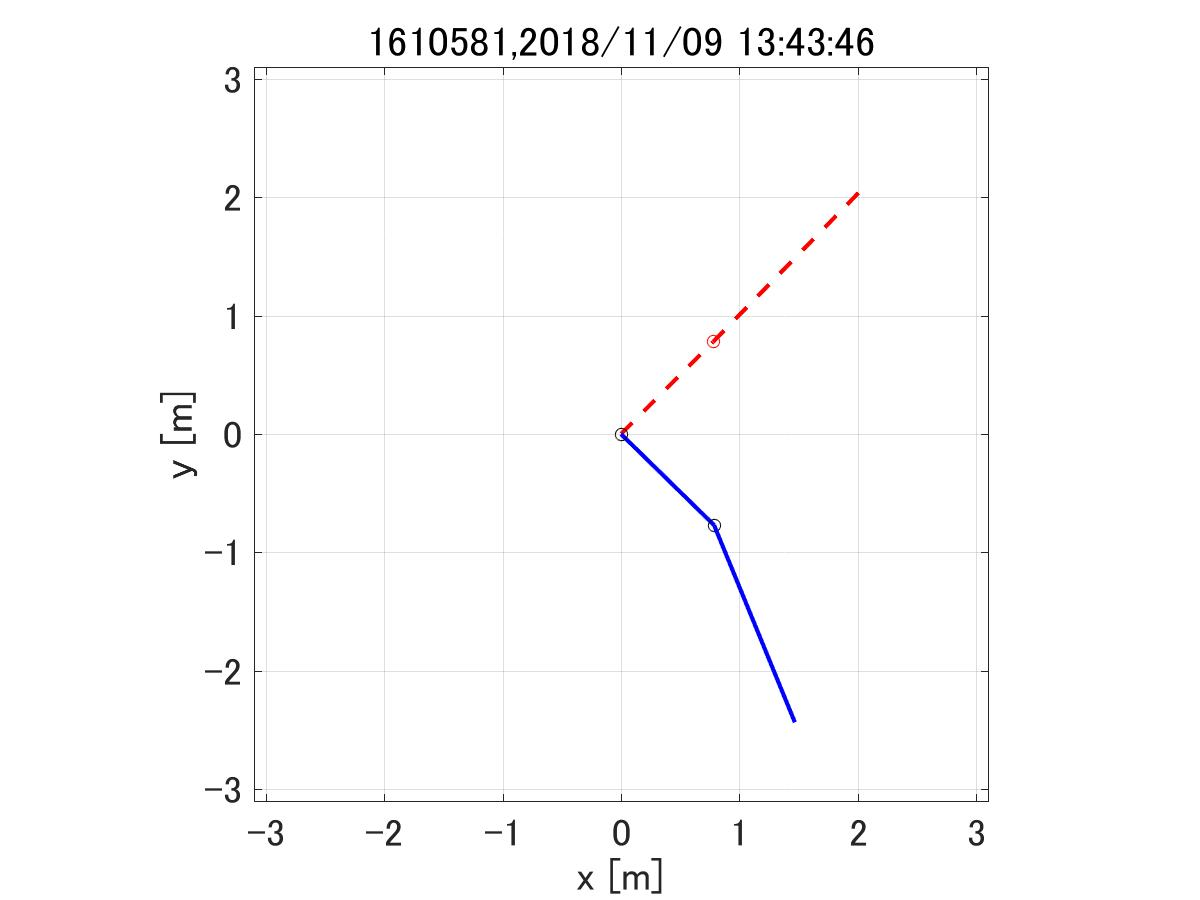
\includegraphics[width=7cm]{../img/img/kansetu_PD_zihen_small_no_model_gosa_saisyu_sisei.jpg}
        \caption{時変のときPD制御を用いてゲインを小,モデル誤差なしと設定したときの最終姿勢.}
      \end{center}
    \end{figure}

    \begin{figure}[H]
      % 図8
      \begin{center}
        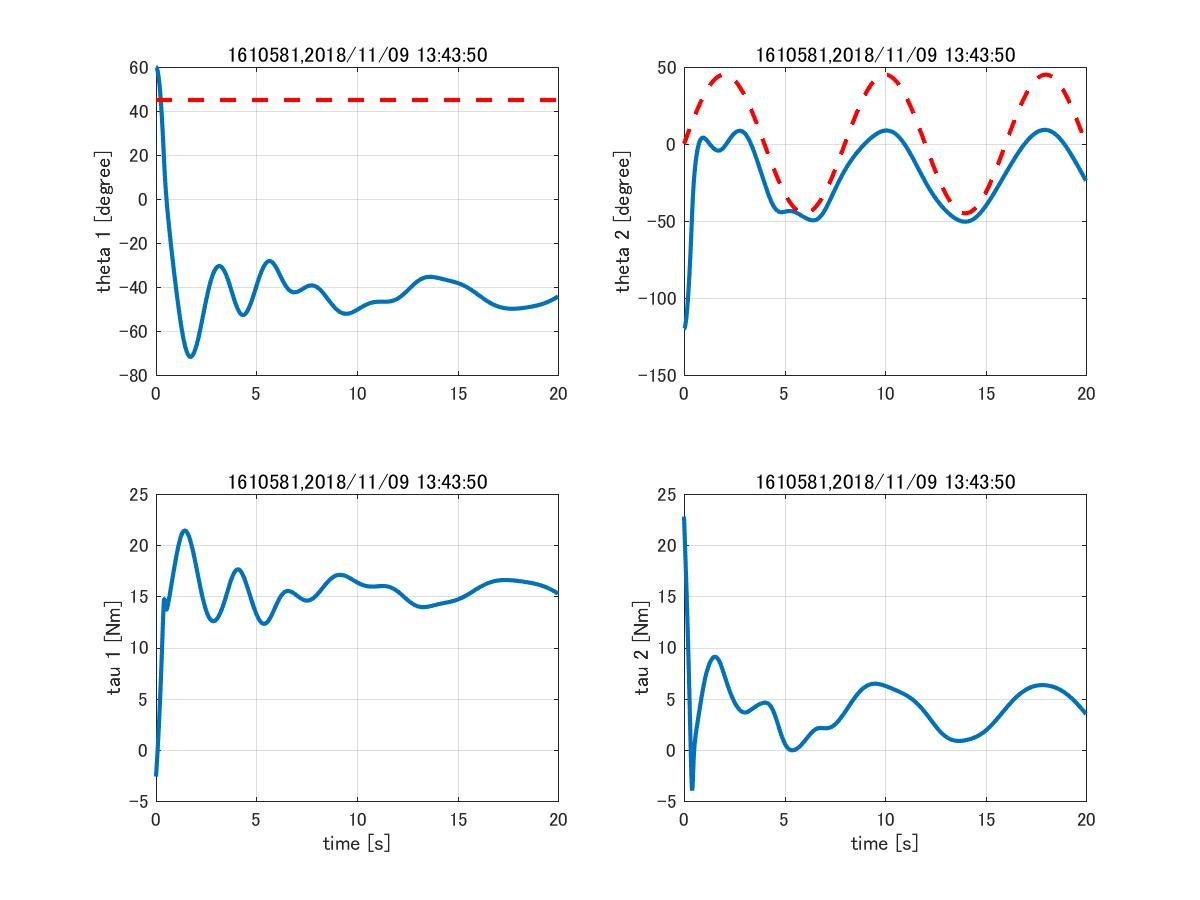
\includegraphics[width=7cm]{../img/img/kansetu_PD_zihen_small_no_model_gosa_zikan_auto.jpg}
        \caption{時変のときPD制御を用いてゲインを小,モデル誤差なしと設定したときの時間応答.}
      \end{center}
    \end{figure}
    %%%%%%%%%%%%%%%%%%%%%%%%%%%%%%%%%%%%%%%%%%%%%%%%%%%%%%%%%%%%%%%%%%%%%%%%%%%%%%%%%%%%%%%%%%%%%%%%%%%
    \begin{figure}[H]
      % 図9
      \begin{center}
        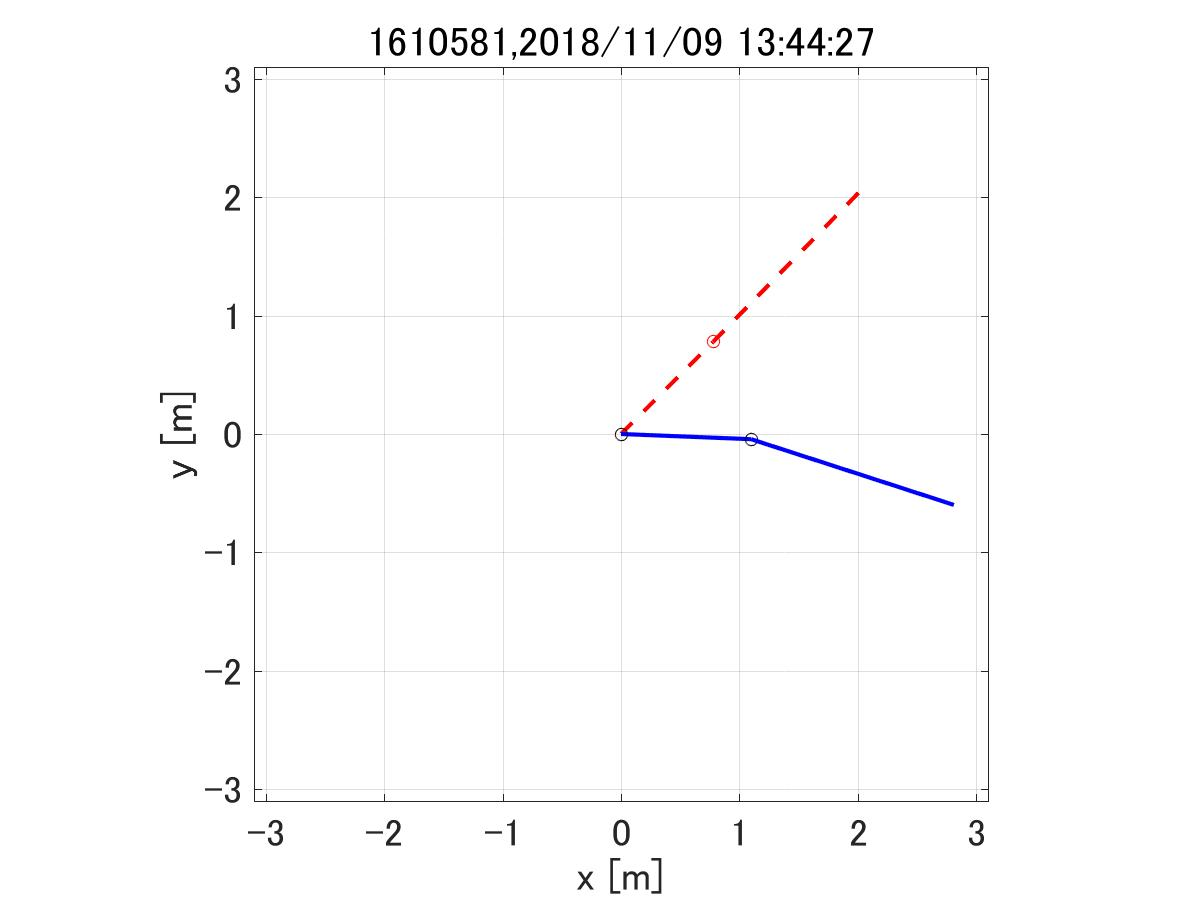
\includegraphics[width=7cm]{../img/img/kansetu_PD_zihen_chu_no_model_gosa_saisyu_sisei.jpg}
        \caption{時変のときPD制御を用いてゲインを中,モデル誤差なしと設定したときの最終姿勢.}
      \end{center}
    \end{figure}

    \begin{figure}[H]
      % 図10
      \begin{center}
        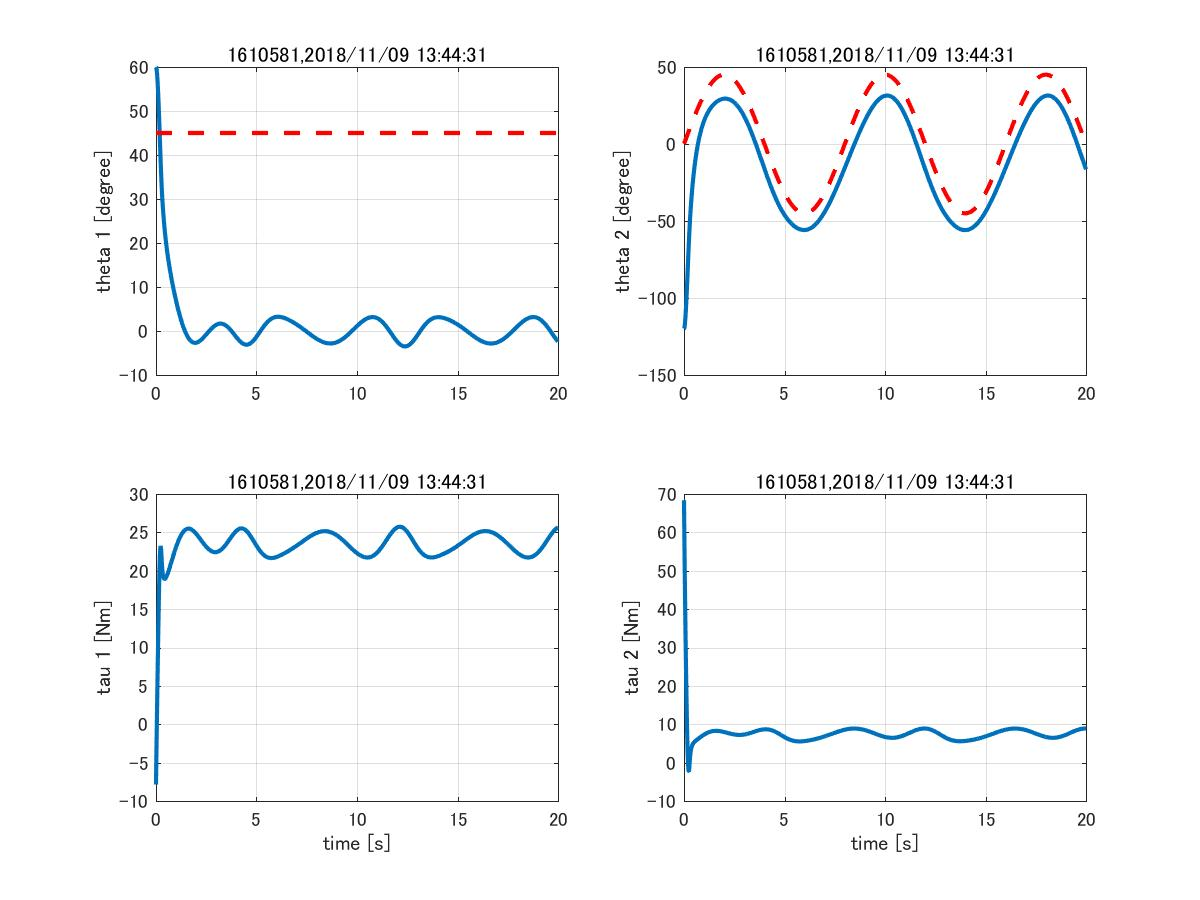
\includegraphics[width=7cm]{../img/img/kansetu_PD_zihen_chu_no_model_gosa_zikan_auto.jpg}
        \caption{時変のときPD制御を用いてゲインを中,モデル誤差なしと設定したときの時間応答.}
      \end{center}
    \end{figure}
    %%%%%%%%%%%%%%%%%%%%%%%%%%%%%%%%%%%%%%%%%%%%%%%%%%%%%%%%%%%%%%%%%%%%%%%%%%%%%%%%%%%%%%%%%%%%%%%%%%%
    \begin{figure}[H]
      % 図11
      \begin{center}
        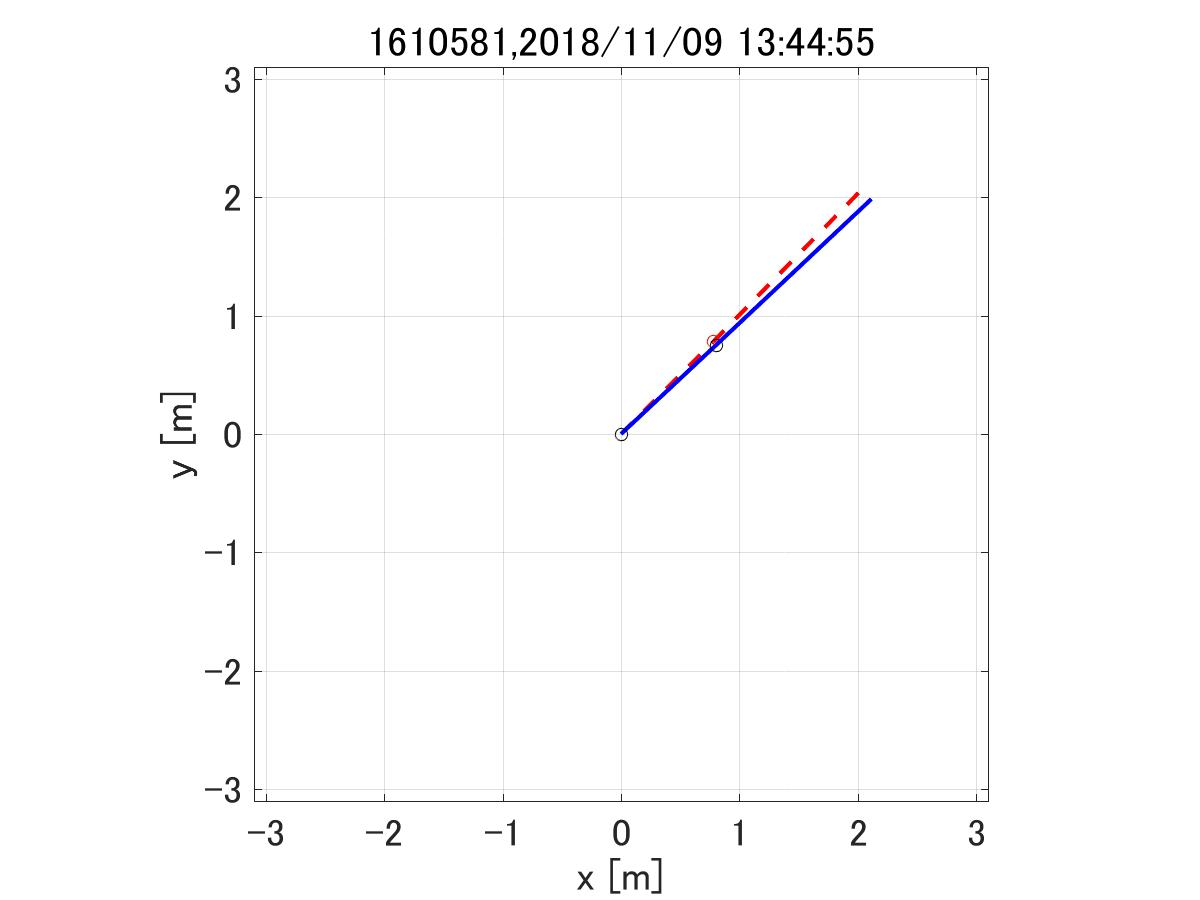
\includegraphics[width=7cm]{../img/img/kansetu_PD_zihen_large_no_model_gosa_saisyu_sisei.jpg}
        \caption{時変のときPD制御を用いてゲインを大,モデル誤差なしと設定したときの最終姿勢.}
      \end{center}
    \end{figure}

    \begin{figure}[H]
      % 図12
      \begin{center}
        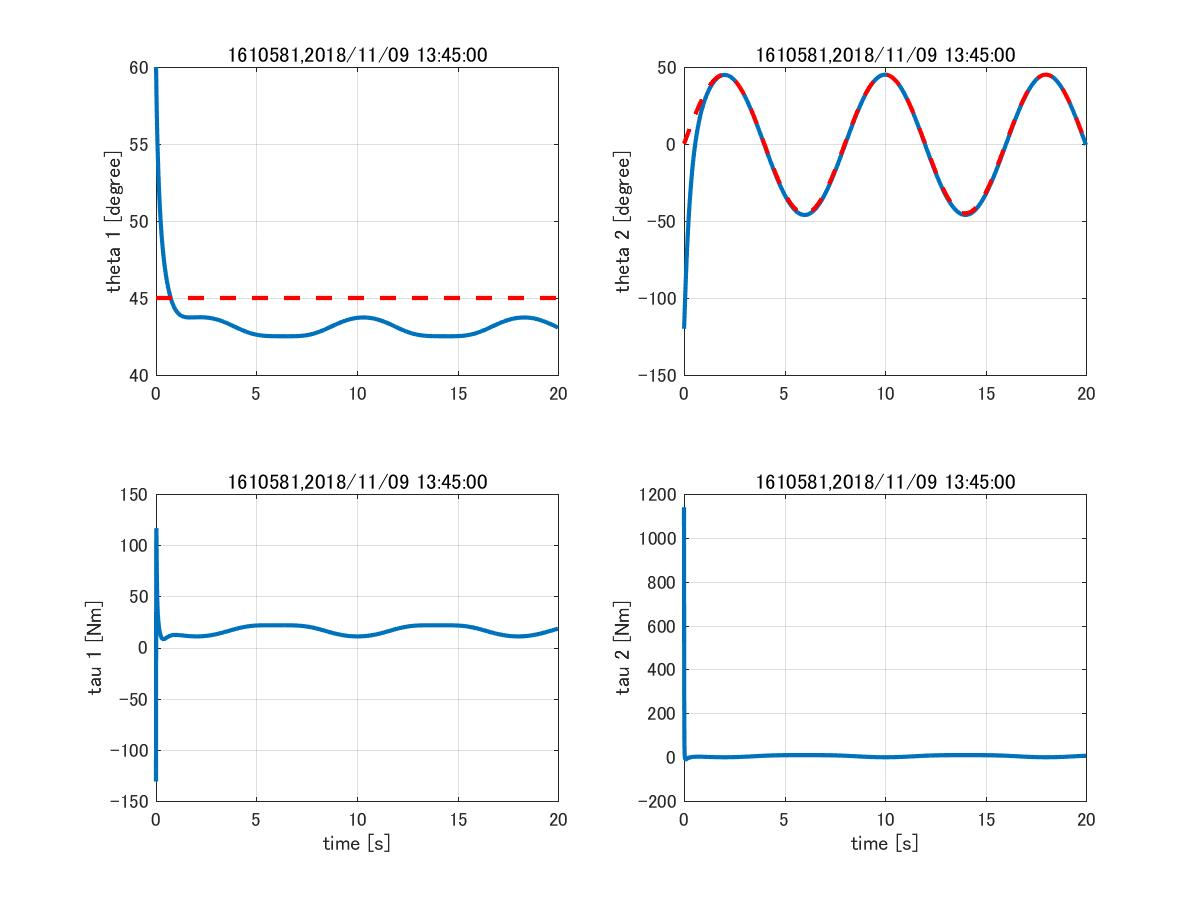
\includegraphics[width=7cm]{../img/img/kansetu_PD_zihen_large_no_model_gosa_zikan_auto.jpg}
        \caption{時変のときPD制御を用いてゲインを大,モデル誤差なしと設定したときの時間応答.}
      \end{center}
    \end{figure}
    %%%%%%%%%%%%%%%%%%%%%%%%%%%%%%%%%%%%%%%%%%%%%%%%%%%%%%%%%%%%%%%%%%%%%%%%%%%%%%%%%%%%%%%%%%%%%%%%%%%
    \begin{figure}[H]
      % 図11
      \begin{center}
        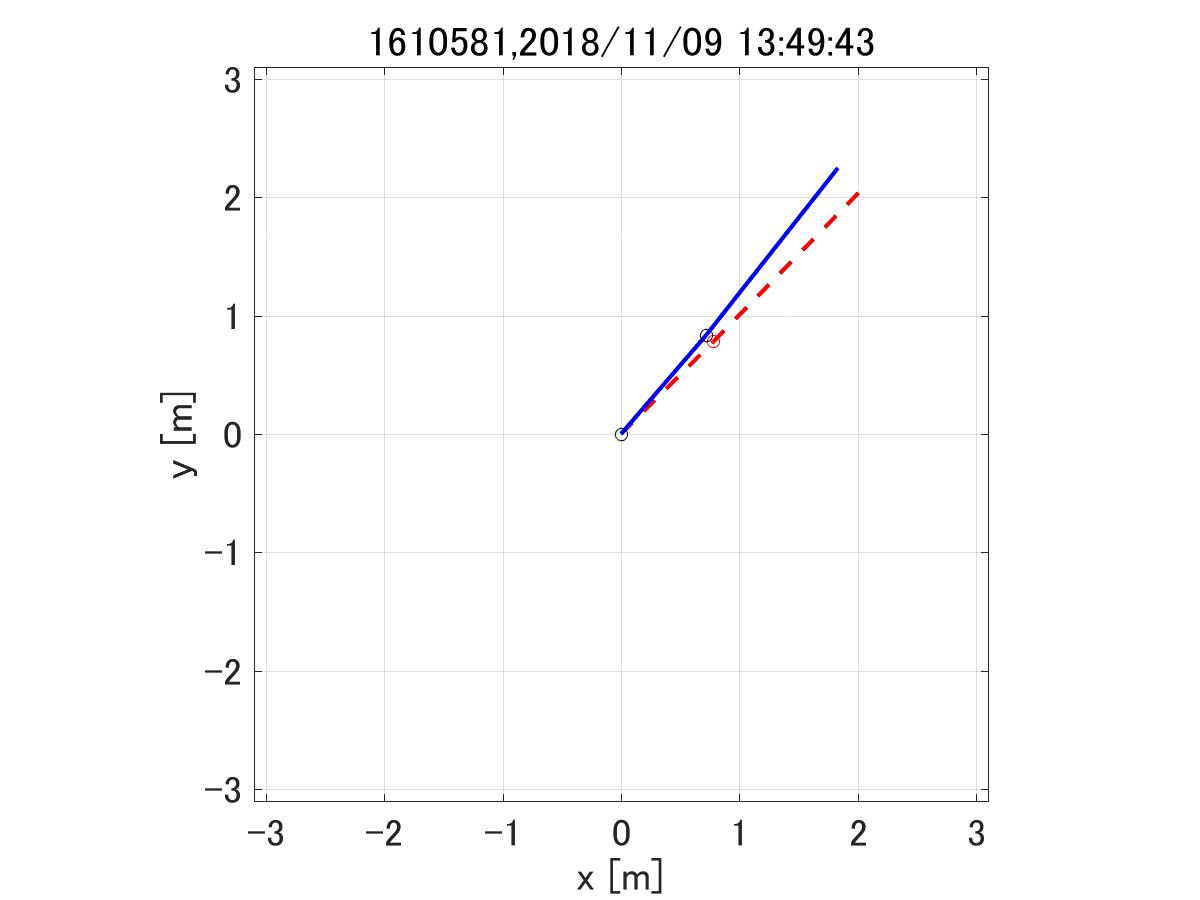
\includegraphics[width=7cm]{../img/img/kansetu_juryoku_hosyo_PD_zihen_small_no_model_gosa_saisyu_sisei.jpg}
        \caption{時変のとき重力補償つきPD制御を用いてゲインを小,モデル誤差なしと設定したときの最終姿勢.}
      \end{center}
    \end{figure}

    \begin{figure}[H]
      % 図12
      \begin{center}
        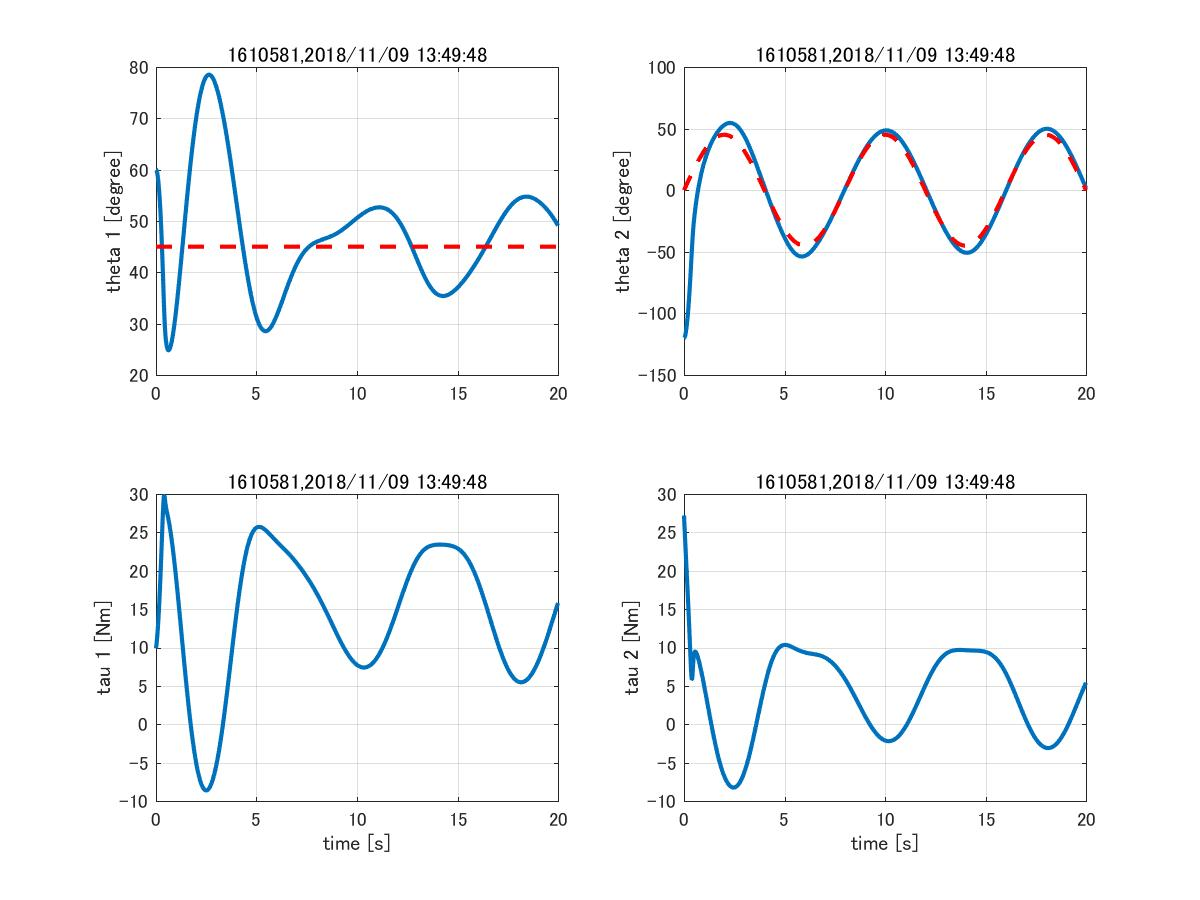
\includegraphics[width=7cm]{../img/img/kansetu_juryoku_hosyo_PD_zihen_small_no_model_gosa_zikan_auto.jpg}
        \caption{時変のとき重力補償つきPD制御を用いてゲインを小,モデル誤差なしと設定したときの時間応答.}
      \end{center}
    \end{figure}
    %%%%%%%%%%%%%%%%%%%%%%%%%%%%%%%%%%%%%%%%%%%%%%%%%%%%%%%%%%%%%%%%%%%%%%%%%%%%%%%%%%%%%%%%%%%%%%%%%%%
    \begin{figure}[H]
      % 図11
      \begin{center}
        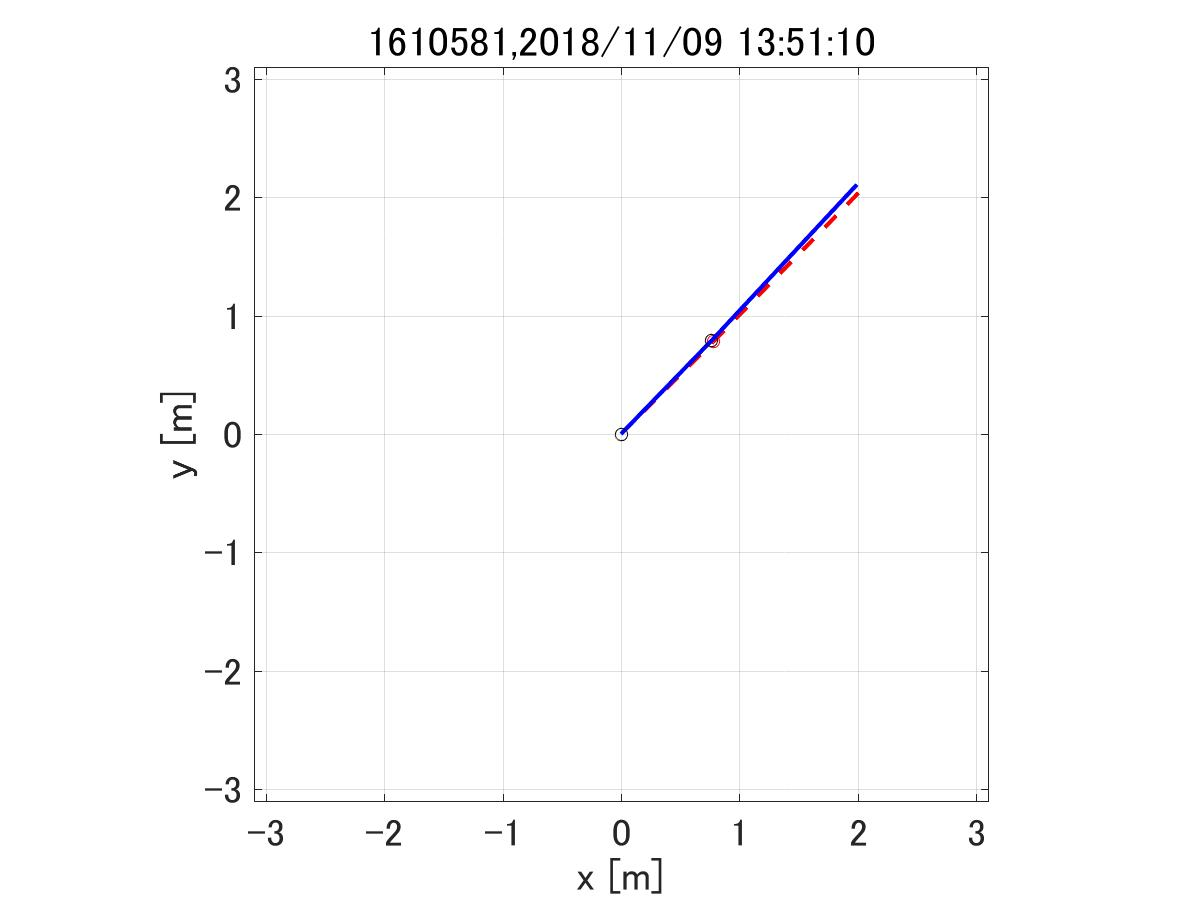
\includegraphics[width=7cm]{../img/img/kansetu_juryoku_hosyo_PD_zihen_chu_no_model_gosa_saisyu_sisei.jpg}
        \caption{時変のとき重力補償つきPD制御を用いてゲインを中,モデル誤差なしと設定したときの最終姿勢.}
      \end{center}
    \end{figure}

    \begin{figure}[H]
      % 図12
      \begin{center}
        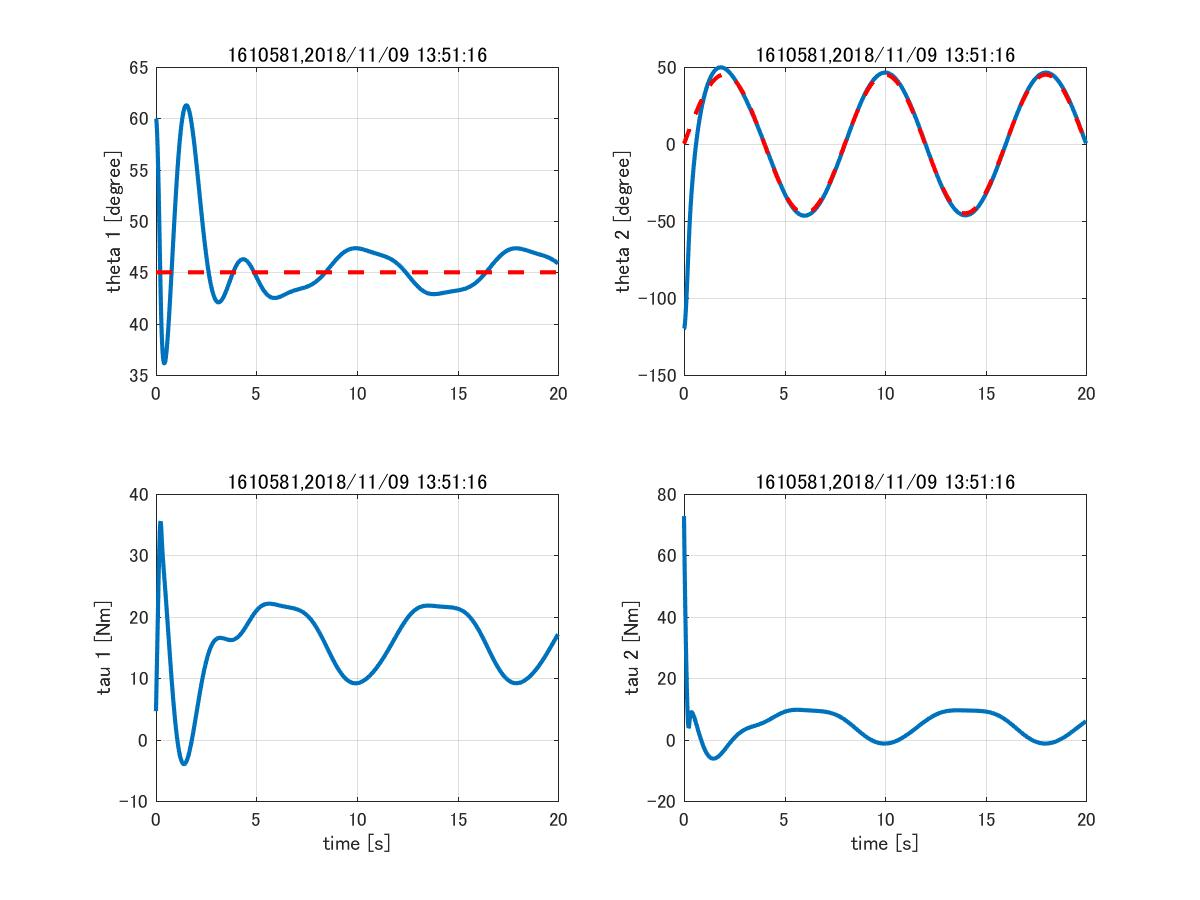
\includegraphics[width=7cm]{../img/img/kansetu_juryoku_hosyo_PD_zihen_chu_no_model_gosa_zikan_auto.jpg}
        \caption{時変のとき重力補償つきPD制御を用いてゲインを中,モデル誤差なしと設定したときの時間応答.}
      \end{center}
    \end{figure}
    %%%%%%%%%%%%%%%%%%%%%%%%%%%%%%%%%%%%%%%%%%%%%%%%%%%%%%%%%%%%%%%%%%%%%%%%%%%%%%%%%%%%%%%%%%%%%%%%%%%
    \begin{figure}[H]
      % 図11
      \begin{center}
        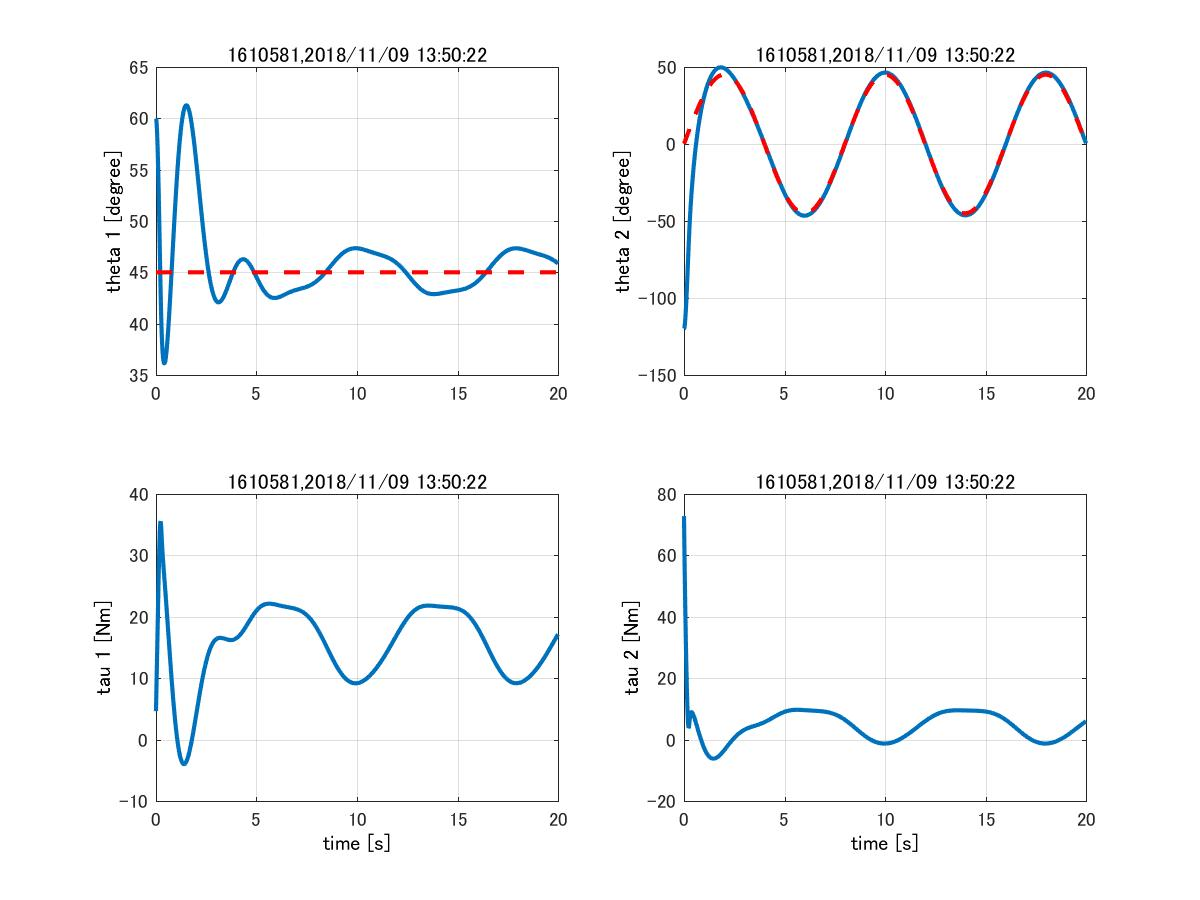
\includegraphics[width=7cm]{../img/img/kansetu_juryoku_hosyo_PD_zihen_large_no_model_gosa_saisyu_sisei.jpg}
        \caption{時変のとき重力補償つきPD制御を用いてゲインを大,モデル誤差なしと設定したときの最終姿勢.}
      \end{center}
    \end{figure}

    \begin{figure}[H]
      % 図12
      \begin{center}
        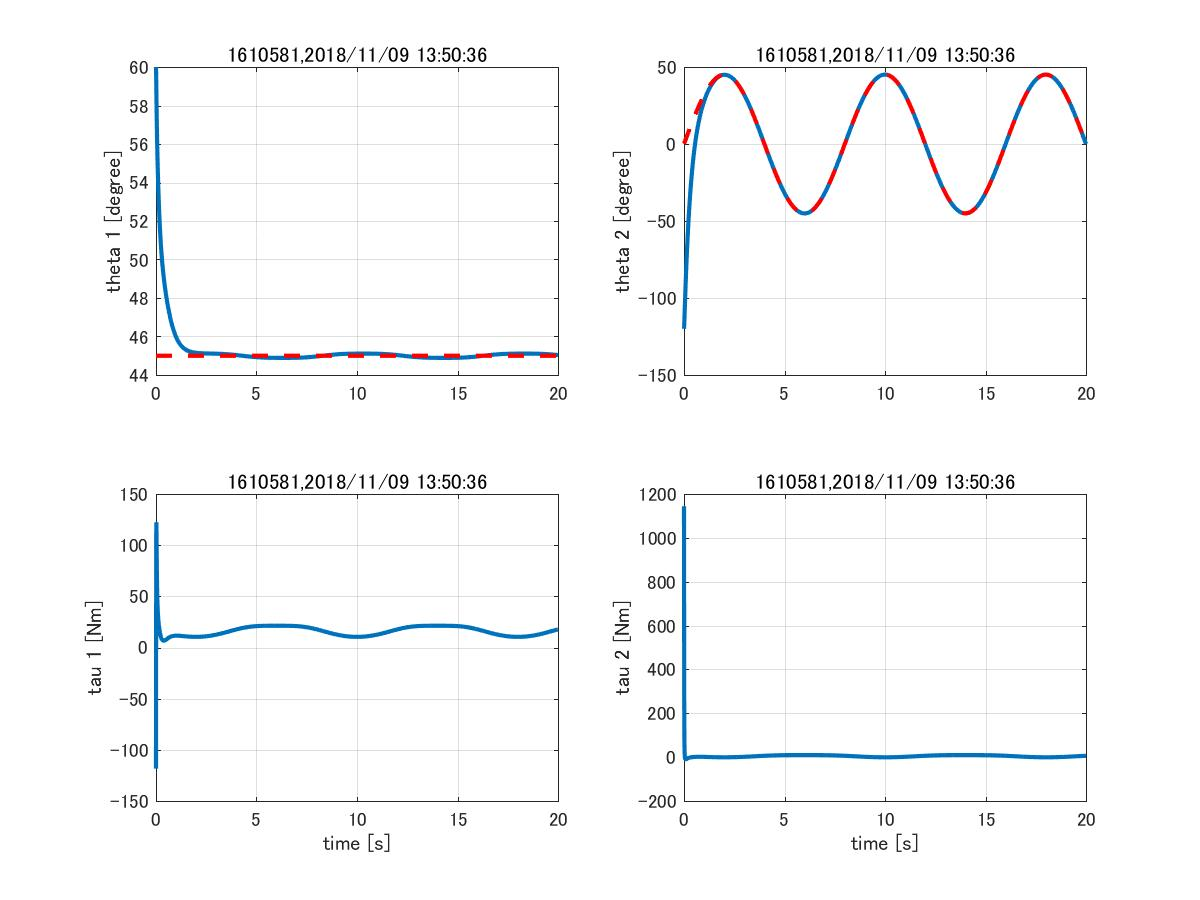
\includegraphics[width=7cm]{../img/img/kansetu_juryoku_hosyo_PD_zihen_large_no_model_gosa_zikan_auto.jpg}
        \caption{時変のとき重力補償つきPD制御を用いてゲインを大,モデル誤差なしと設定したときの時間応答.}
      \end{center}
    \end{figure}
    %%%%%%%%%%%%%%%%%%%%%%%%%%%%%%%%%%%%%%%%%%%%%%%%%%%%%%%%%%%%%%%%%%%%%%%%%%%%%%%%%%%%%%%%%%%%%%%%%%%
    \begin{figure}[H]
      % 図11
      \begin{center}
        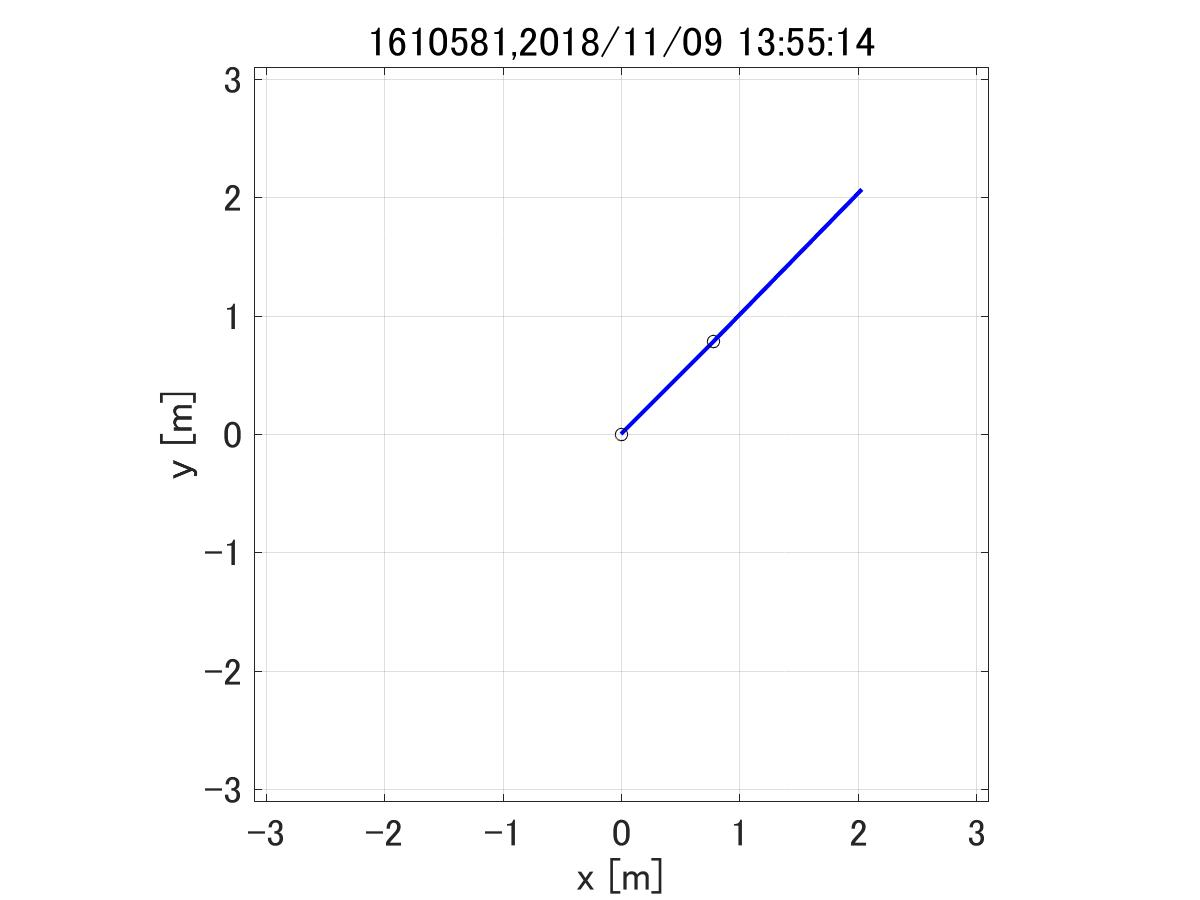
\includegraphics[width=7cm]{../img/img/kansetu_FB_zihen_small_no_model_gosa_saisyu_sisei.jpg}
        \caption{時変のときフィードバック線形化制御を用いてゲインを小,モデル誤差なしと設定したときの最終姿勢.}
      \end{center}
    \end{figure}

    \begin{figure}[H]
      % 図12
      \begin{center}
        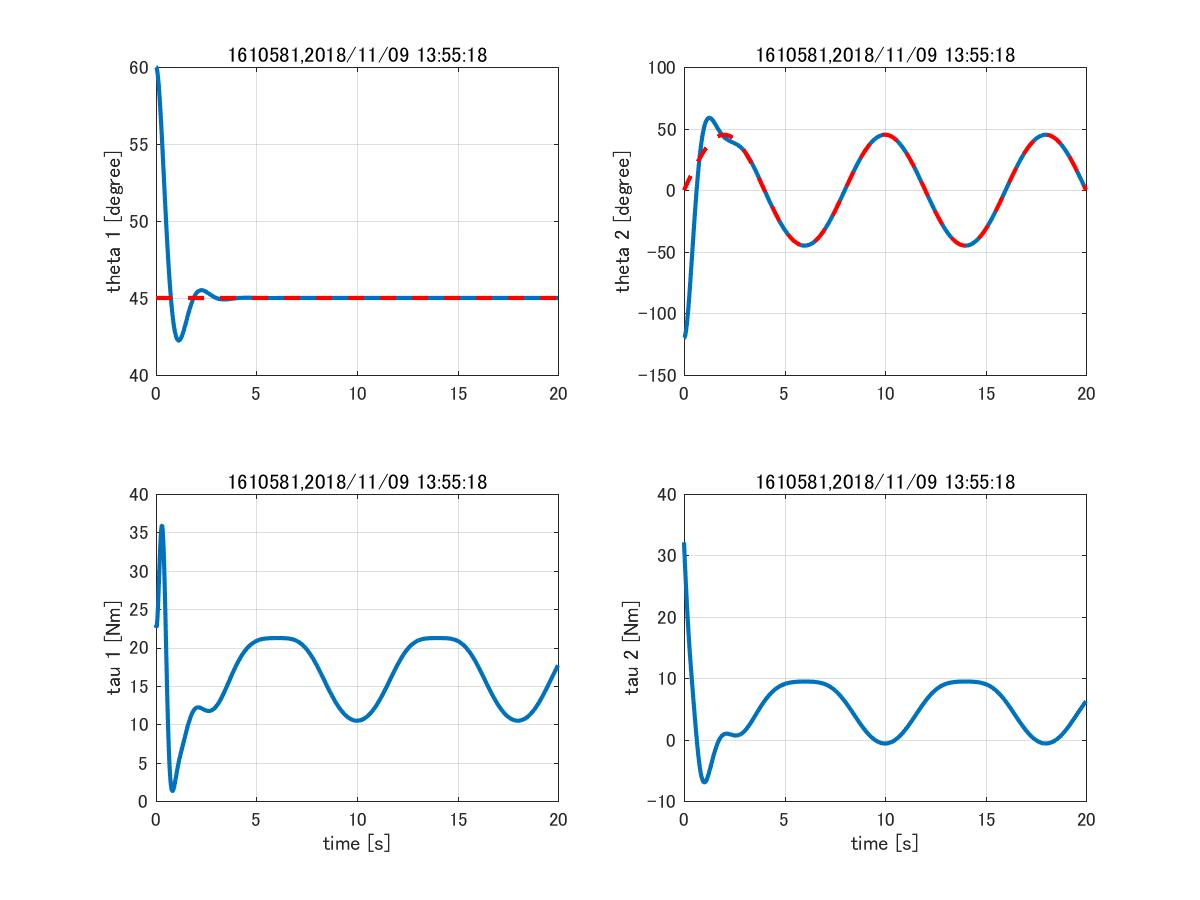
\includegraphics[width=7cm]{../img/img/kansetu_FB_zihen_small_no_model_gosa_zikan_auto.jpg}
        \caption{時変のときフィードバック線形化制御を用いてゲインを小,モデル誤差なしと設定したときの時間応答.}
      \end{center}
    \end{figure}
    %%%%%%%%%%%%%%%%%%%%%%%%%%%%%%%%%%%%%%%%%%%%%%%%%%%%%%%%%%%%%%%%%%%%%%%%%%%%%%%%%%%%%%%%%%%%%%%%%%%
    \begin{figure}[H]
      % 図11
      \begin{center}
        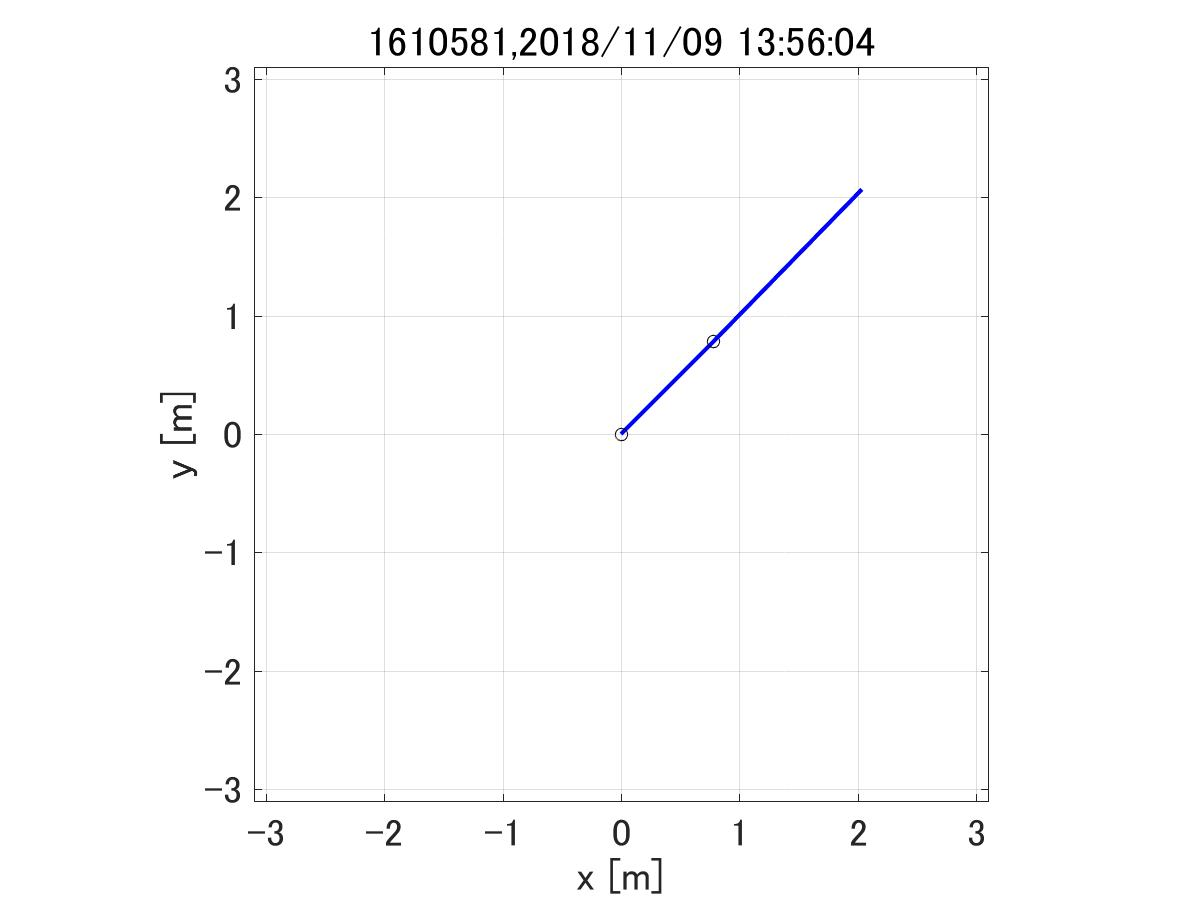
\includegraphics[width=7cm]{../img/img/kansetu_FB_zihen_chu_no_model_gosa_saisyu_sisei.jpg}
        \caption{時変のときフィードバック線形化制御を用いてゲインを中,モデル誤差なしと設定したときの最終姿勢.}
      \end{center}
    \end{figure}

    \begin{figure}[H]
      % 図12
      \begin{center}
        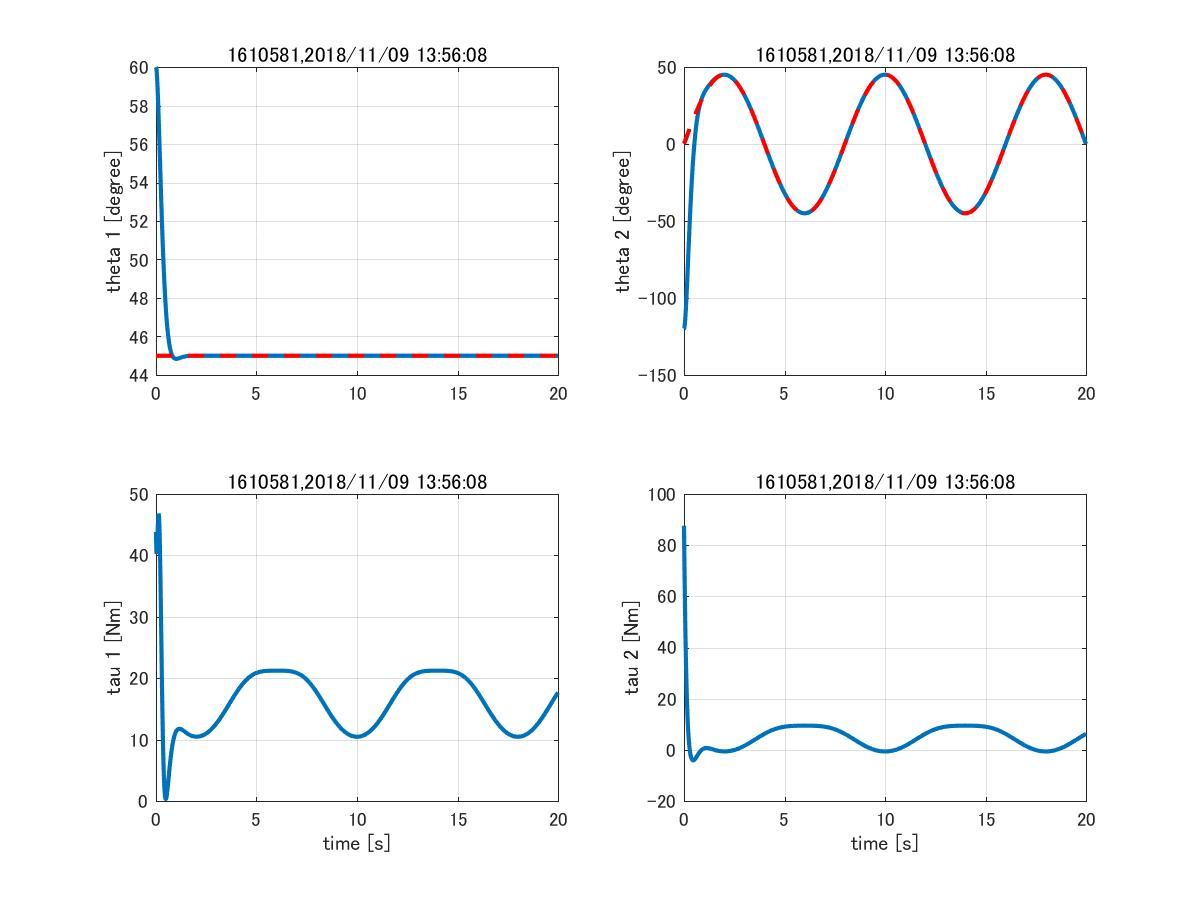
\includegraphics[width=7cm]{../img/img/kansetu_FB_zihen_chu_no_model_gosa_zikan_auto.jpg}
        \caption{時変のときフィードバック線形化制御を用いてゲインを中,モデル誤差なしと設定したときの時間応答.}
      \end{center}
    \end{figure}
    %%%%%%%%%%%%%%%%%%%%%%%%%%%%%%%%%%%%%%%%%%%%%%%%%%%%%%%%%%%%%%%%%%%%%%%%%%%%%%%%%%%%%%%%%%%%%%%%%%%
    \begin{figure}[H]
      % 図11
      \begin{center}
        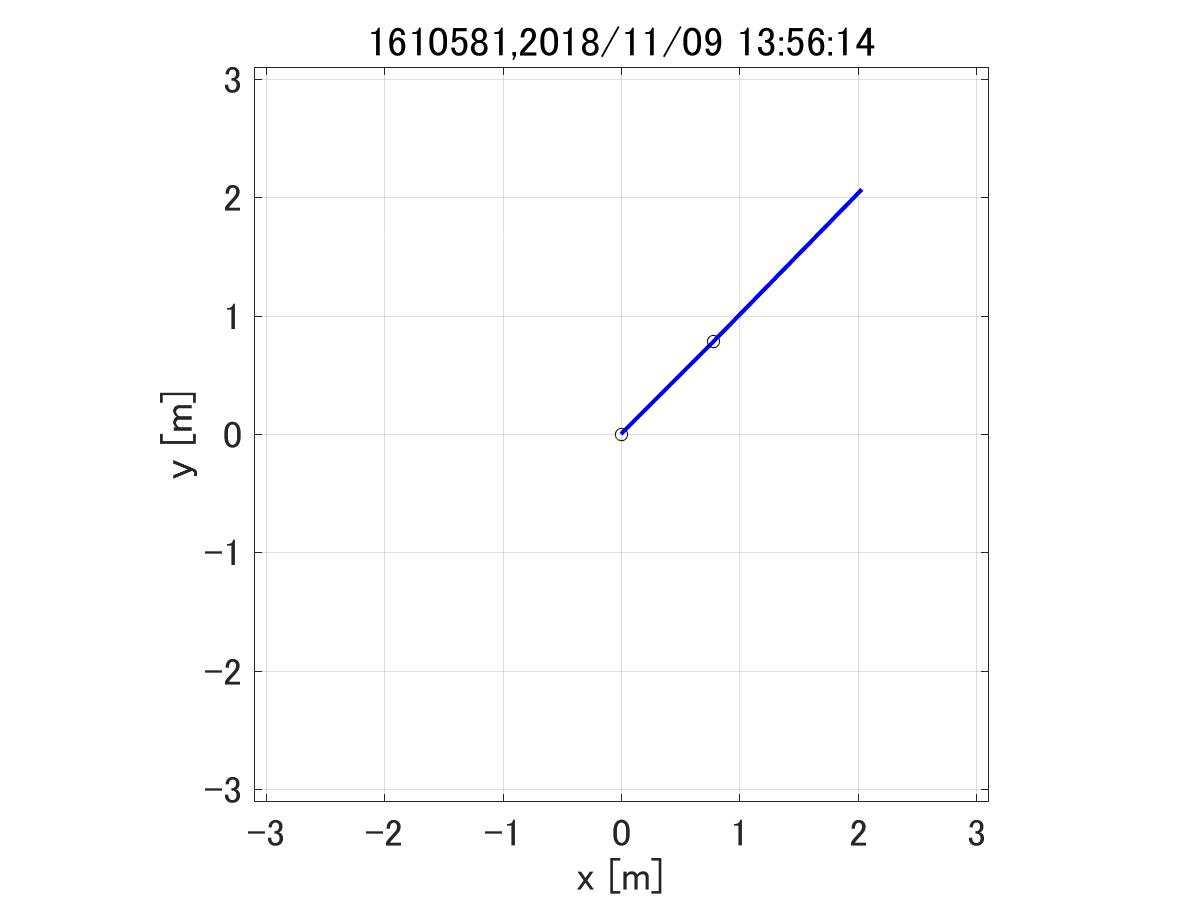
\includegraphics[width=7cm]{../img/img/kansetu_FB_zihen_large_no_model_gosa_saisyu_sisei.jpg}
        \caption{時変のときフィードバック線形化制御を用いてゲインを大,モデル誤差なしと設定したときの最終姿勢.}
      \end{center}
    \end{figure}

    \begin{figure}[H]
      % 図12
      \begin{center}
        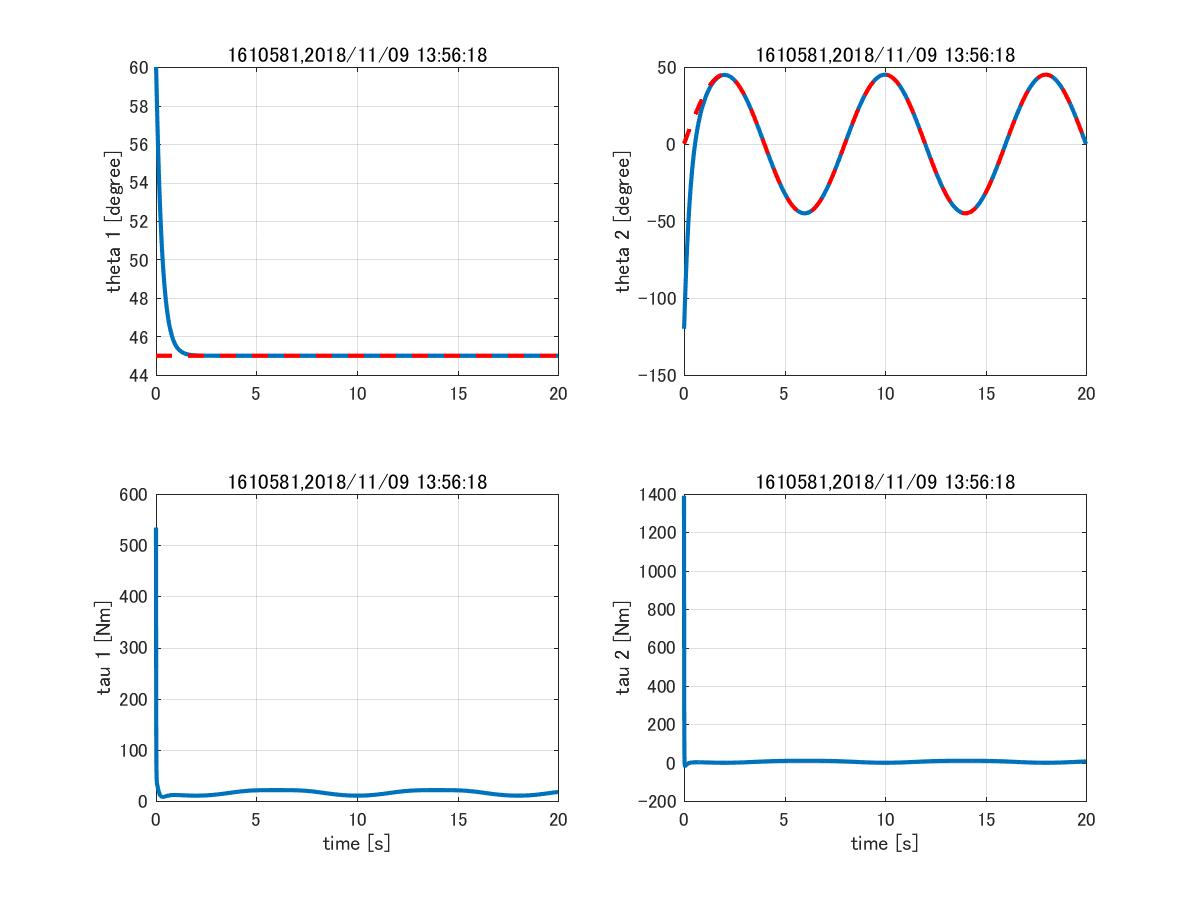
\includegraphics[width=7cm]{../img/img/kansetu_FB_zihen_large_no_model_gosa_zikan_auto.jpg}
        \caption{時変のときフィードバック線形化制御を用いてゲインを大,モデル誤差なしと設定したときの時間応答.}
      \end{center}
    \end{figure}

    \begin{table}[H]
      \begin{center}
        \caption{フィードバック線形化制御におけて,ゲインパラメータの設定でのTauの値. Tauの値は小さいほど良いと評価する.}
        \scalebox{0.8}[0.9] {
          \begin{tabular}{llll}
          ゲインの値 & 小 & 中  & 大 \\ \hline
          Tau1[Nm] & 10-22のsin波 & 10-20のsin波 & 0-1のsin波 \\
          Tau2[Nm] & 0-10のsin波 & 0-10のsin波 & 0
          \end{tabular}
        }
      \end{center}
    \end{table}

  \subsection{課題 3.}
    % 課題3
    課題1,2で良好な結果が得られた制御方法とゲインの組み合わせについて,モデル誤差をありに変更して制御を実行したときの結果を考察する.
    どちらも最終姿勢は目標位置と同じ位置にいる. 結果もモデル誤差なしの時と変わることはなかった. また,より良い結果を得るために岡島ら[2]は
    非線形システムを線形システムとして扱うことによっ
    て,さまざまに提案されている線形システムに対する制御系
    設計法を適用することができると提案している. 本実験では,複雑な非線形システムではないにしろ,線形化への変換効率をあげることがより良い結果
    を得るための方策であると考えた.

    \begin{figure}[H]
      % 図12
      \begin{center}
        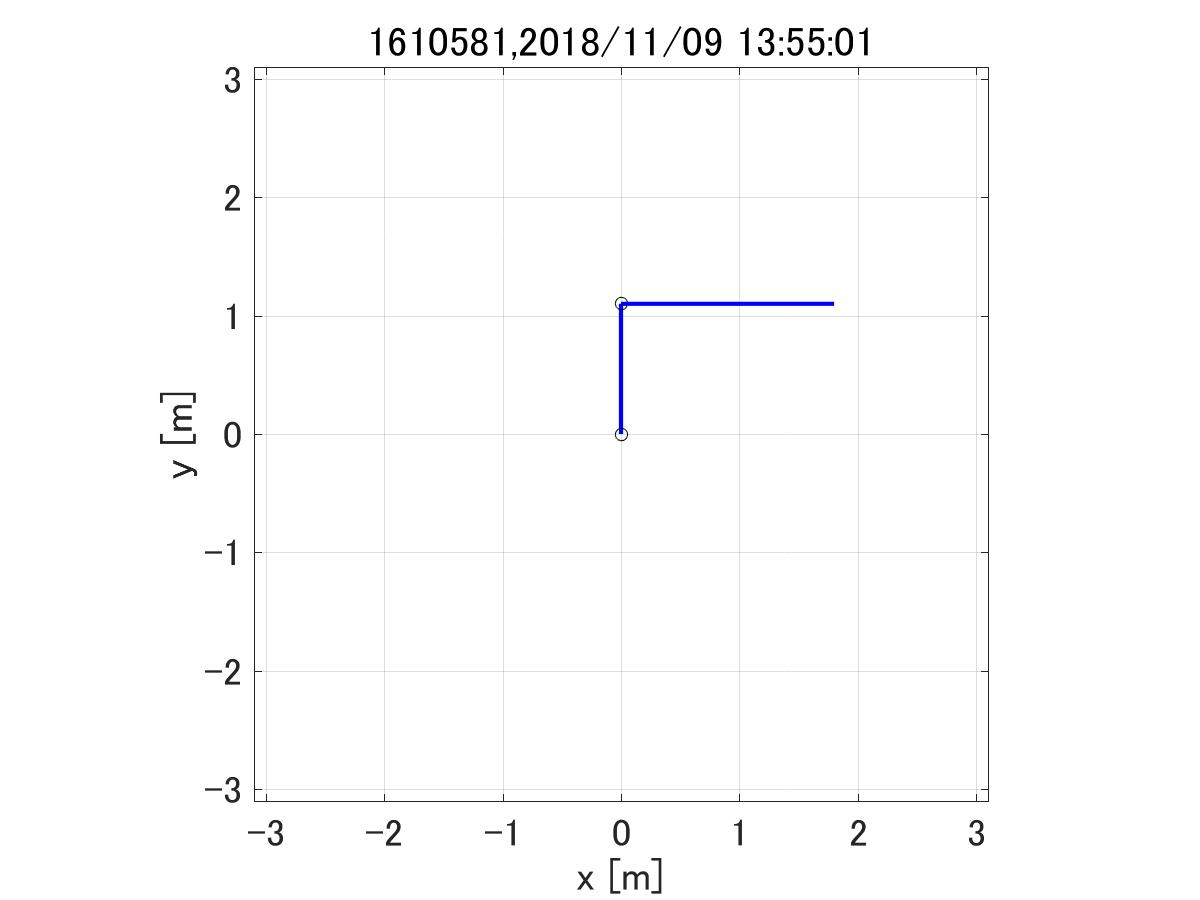
\includegraphics[width=7cm]{../img/img/kansetu_FB_zifuhen_large_yes_model_gosa_saisyu_sisei.jpg}
        \caption{時不変のときフィードバック線形化制御を用いてゲインを大,モデル誤差ありと設定したときの最終姿勢.}
      \end{center}
    \end{figure}

    \begin{figure}[H]
      % 図12
      \begin{center}
        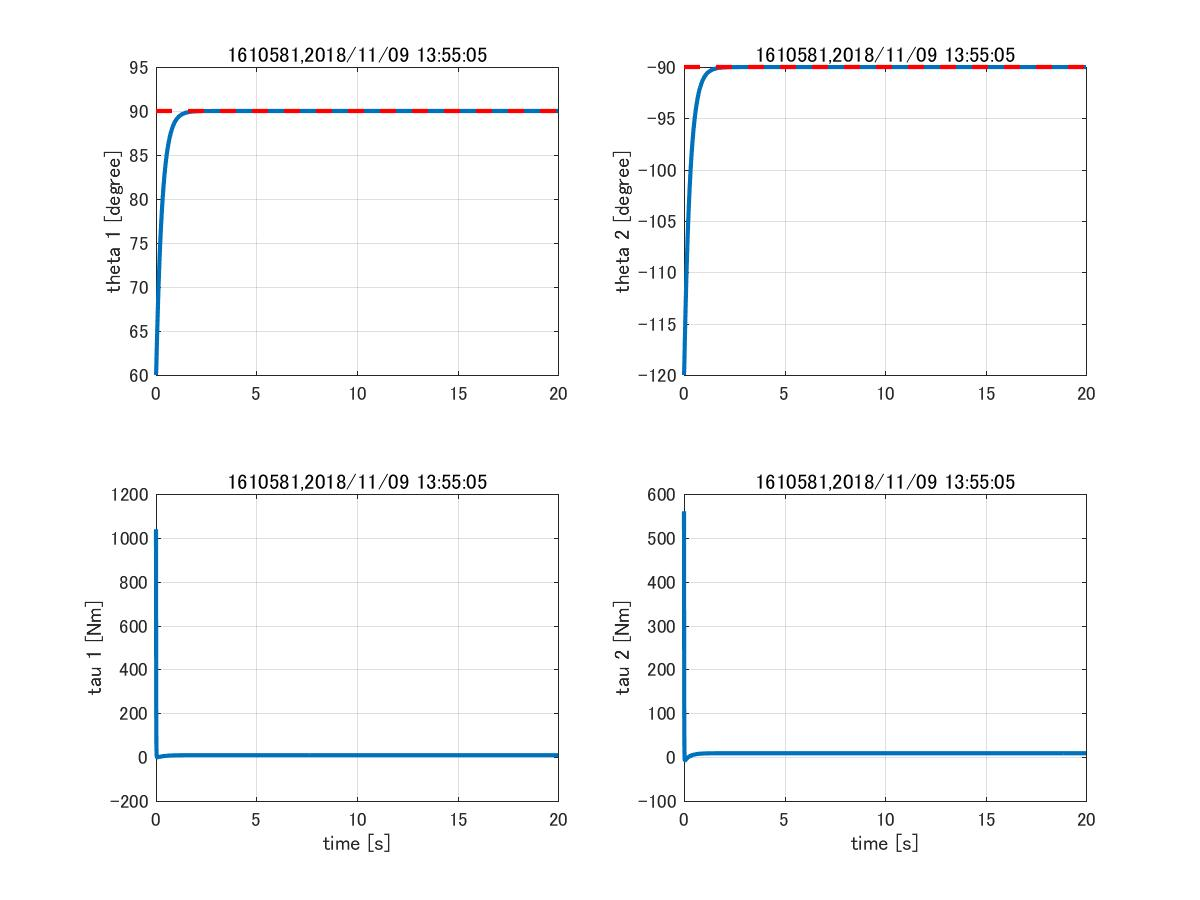
\includegraphics[width=7cm]{../img/img/kansetu_FB_zifuhen_large_yes_model_gosa_zikan_auto.jpg}
        \caption{時不変のときフィードバック線形化制御を用いてゲインを大,モデル誤差ありと設定したときの時間応答.}
      \end{center}
    \end{figure}

    \begin{figure}[H]
      % 図12
      \begin{center}
        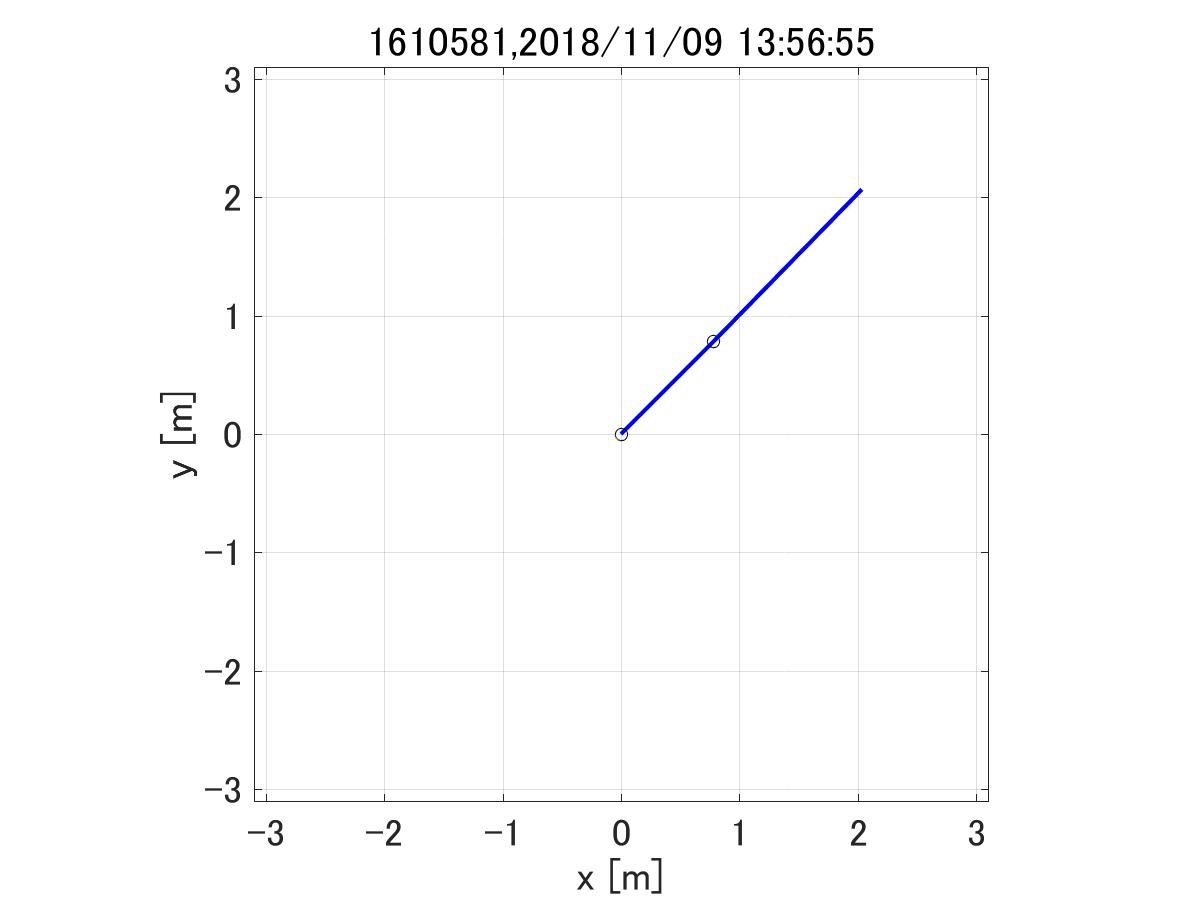
\includegraphics[width=7cm]{../img/img/kansetu_FB_zihen_large_yes_model_gosa_saisyu_sisei.jpg}
        \caption{時変のときフィードバック線形化制御を用いてゲインを大,モデル誤差ありと設定したときの最終姿勢.}
      \end{center}
    \end{figure}
    
    \begin{figure}[H]
      % 図12
      \begin{center}
        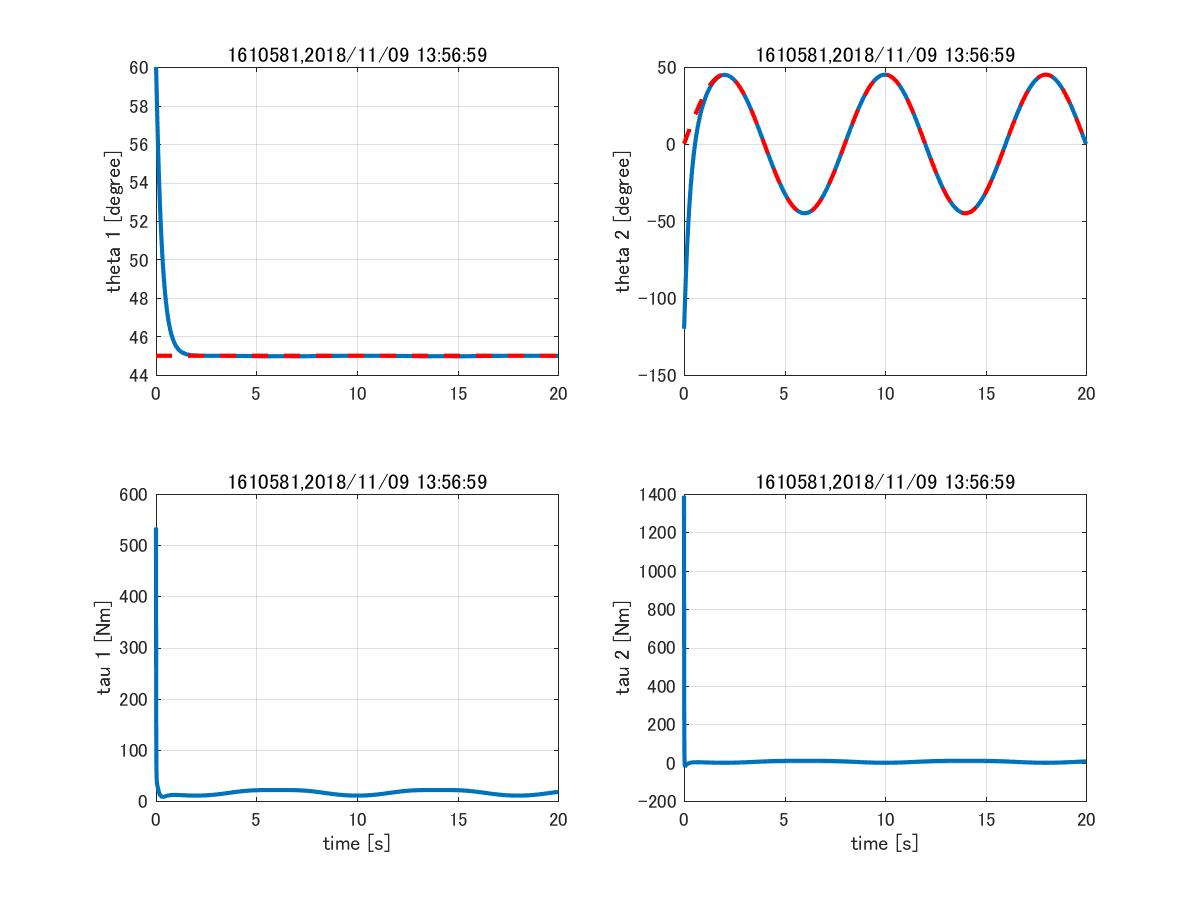
\includegraphics[width=7cm]{../img/img/kansetu_FB_zihen_large_yes_model_gosa_zikan_auto.jpg}
        \caption{時変のときフィードバック線形化制御を用いてゲインを大,モデル誤差ありと設定したときの時間応答.}
      \end{center}
    \end{figure}

  \subsection{課題 4.}
    % 課題4
    2リンクアームを対象に,各種目標値での制御を実行して結果を考察する. 数値シミュレーションと実機での結果を図41 $\to$ 54に示す.
    \begin{enumerate}
      \item 各種目標値と制御結果の関係についての考察.
        どちらも目標値には収束していることがわかる. また,時間軸でグラフを見たときに,どのラインも相関があることがわかる.

      \item シミュレーションと実機の結果を比較し考察.
        実機ではシミュレーションに比べ,最終的な到達地点は変わらないが,目標位置へと早く到達していることがわかる. つまり,実機の方が無駄な動きが多いと言うことである.
        また,図46のdtheta-time図を見ると,値が急に爆発している箇所がある. これはロボットアームの稼働域からはみ出るような動きをしようとすると,正常に値が計測できなかったためだと考えられる.
  [3]によると,この点が特異点であるので,逆運動学計算の解求めることができないから生じたと考えられる. 例えば一直線上に並んで伸びきった姿勢でよく見られる.
        図53, 54では実際に上記の問題となる位置で動作した結果を示しているが,同様な動きがこれら二つの結果にも現れている.

        \begin{figure}[H]
          % 図12
          \begin{center}
            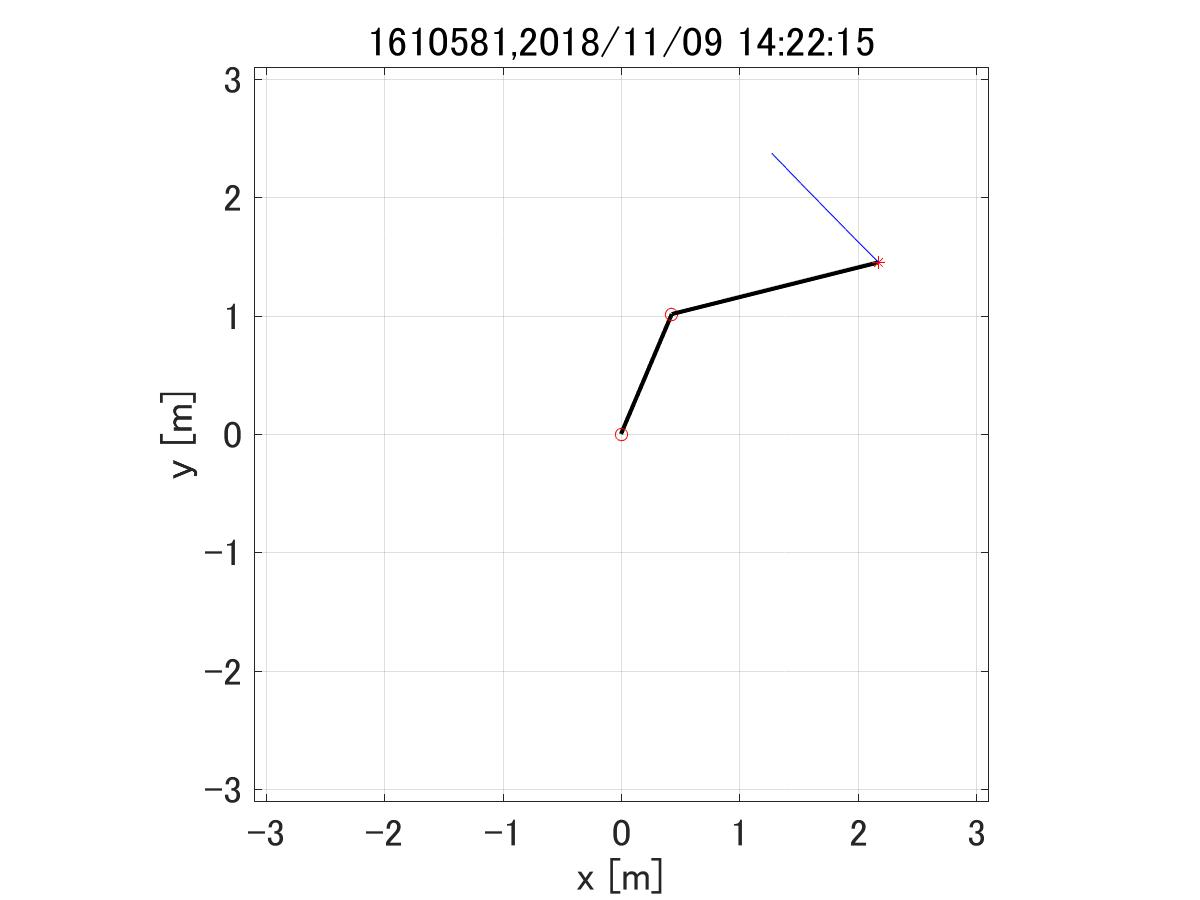
\includegraphics[width=7cm]{../img/kadai45/jpg_hand_zifuhen_saisyu_sisei.jpg}
            \caption{時不変のときの数値シミュレーションにおける最終姿勢.}
          \end{center}
        \end{figure}
        
        \begin{figure}[H]
          % 図12
          \begin{center}
            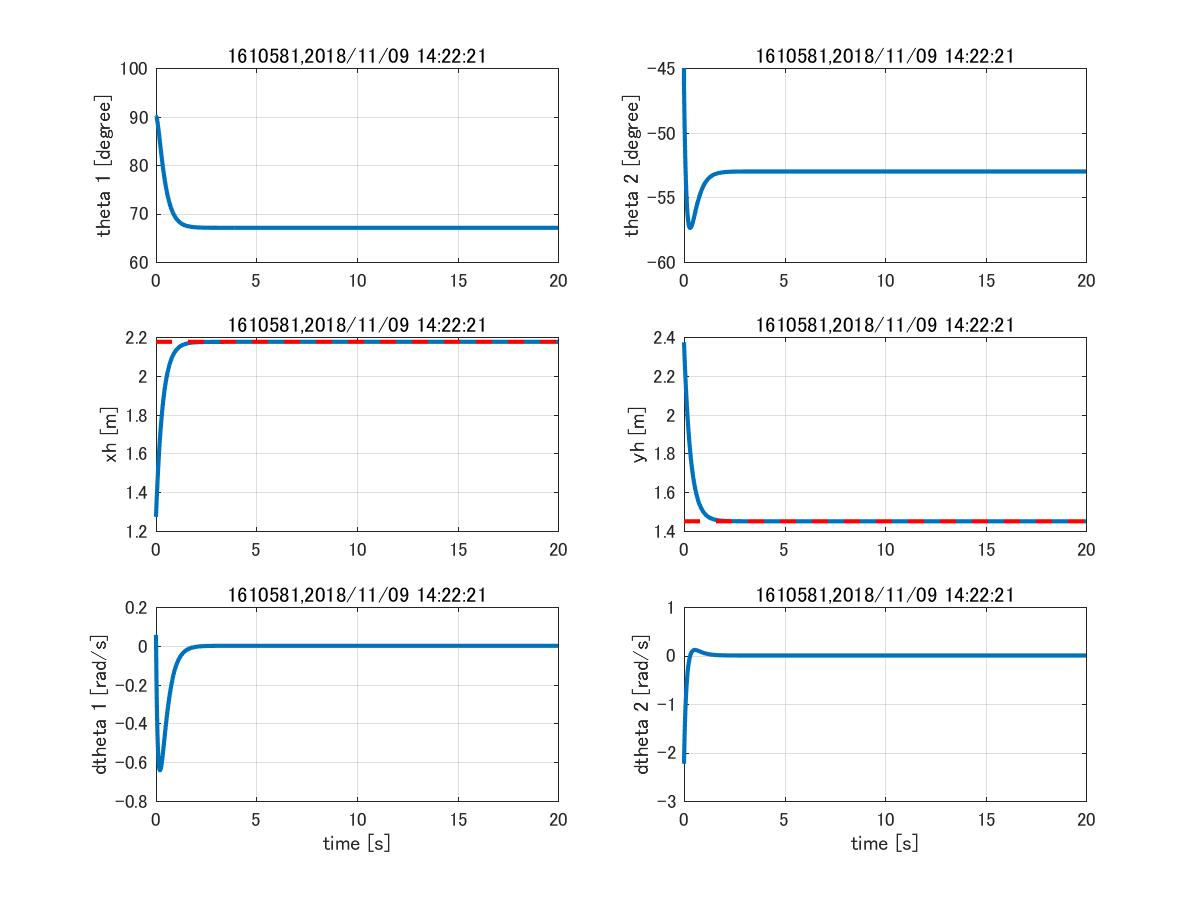
\includegraphics[width=7cm]{../img/kadai45/jpg_hand_zifuhen_auto_zikan.jpg}
            \caption{時不変のときの数値シミュレーションにおける応答時間.}
          \end{center}
        \end{figure}
        %%%%%%%%%%%%%%%%%%%%%%%%%%%%%%%%%%%%%%%%%%%%%%%%%%%%%%%%%%%%%%%%%%%%%%%%%%%%%%%%%
        \begin{figure}[H]
          % 図12
          \begin{center}
            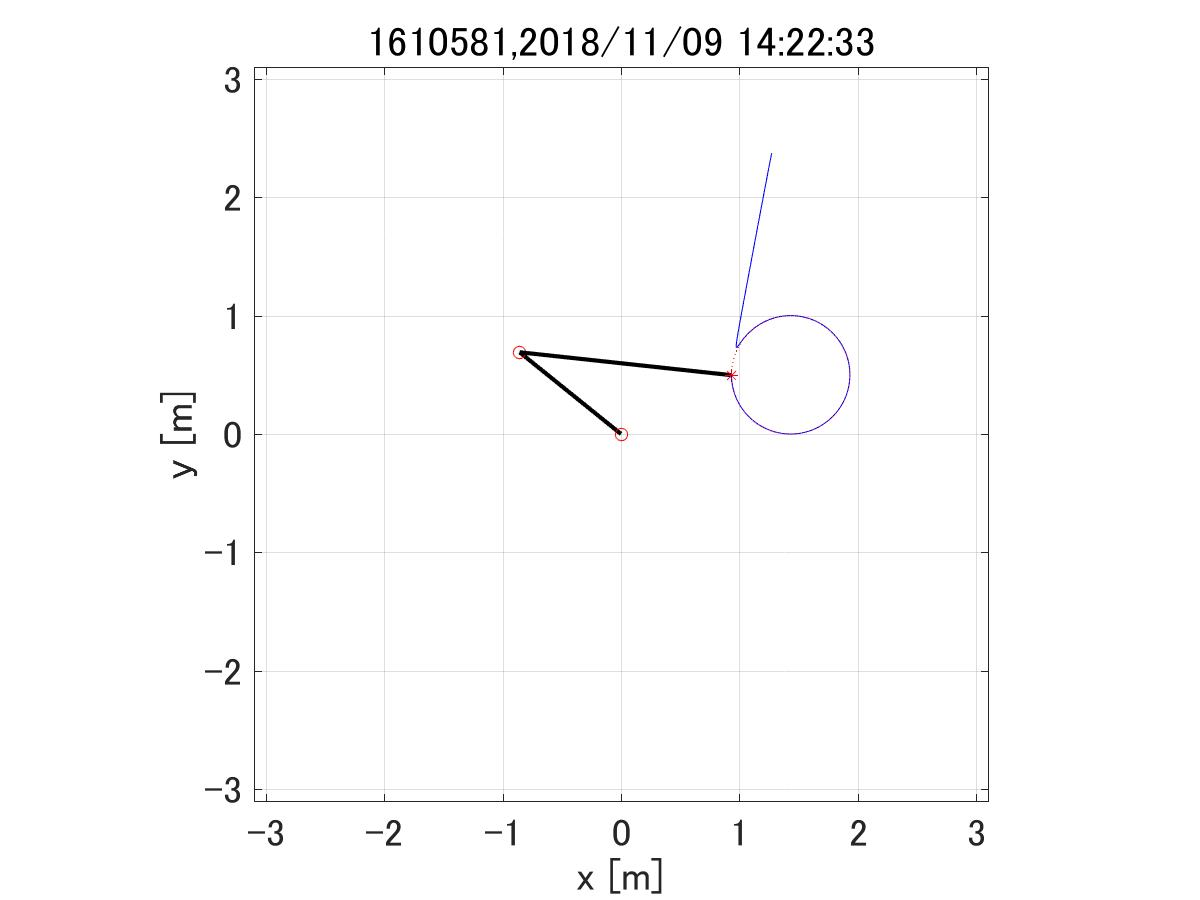
\includegraphics[width=7cm]{../img/kadai45/jpg_hand_zihen_saisyu_sise_1.jpg}
            \caption{時変1のときの数値シミュレーションにおける最終姿勢.}
          \end{center}
        \end{figure}
        
        \begin{figure}[H]
          % 図12
          \begin{center}
            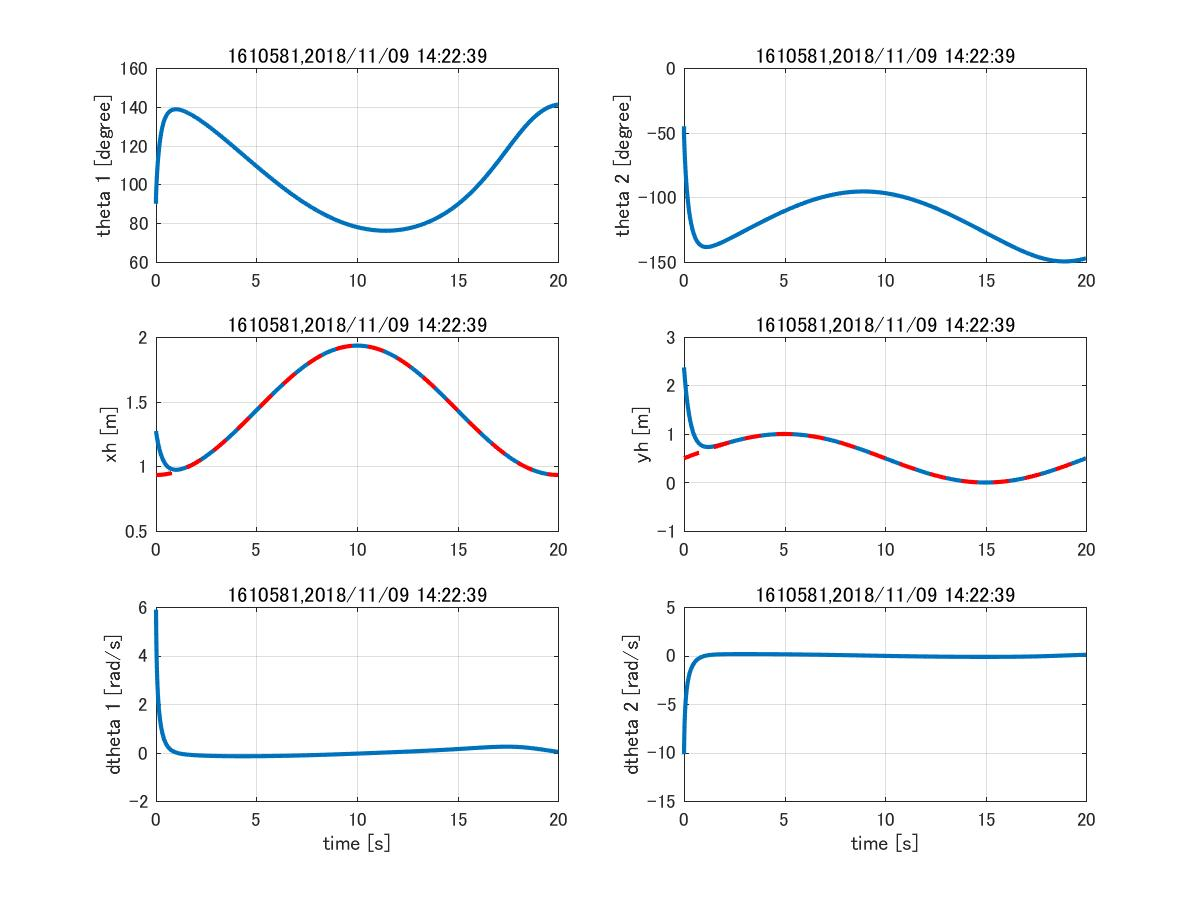
\includegraphics[width=7cm]{../img/kadai45/jpg_hand_zihen_auto_zikan_1.jpg}
            \caption{時変1のときの数値シミュレーションにおける応答時間.}
          \end{center}
        \end{figure}
        %%%%%%%%%%%%%%%%%%%%%%%%%%%%%%%%%%%%%%%%%%%%%%%%%%%%%%%%%%%%%%%%%%%%%%%%%%%%%%%%%
        \begin{figure}[H]
          % 図12
          \begin{center}
            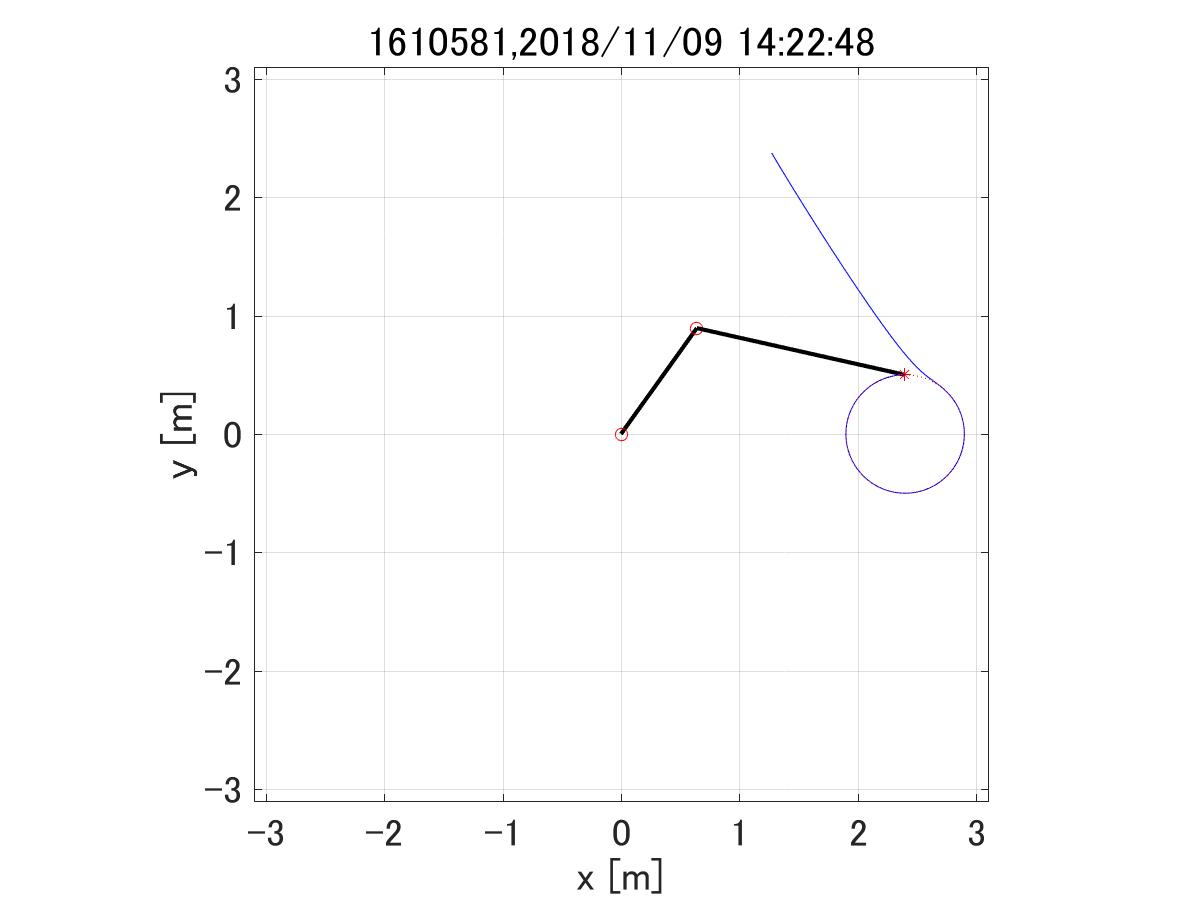
\includegraphics[width=7cm]{../img/kadai45/jpg_hand_zihen_saisyu_sise_2.jpg}
            \caption{時変2のときの数値シミュレーションにおける最終姿勢.}
          \end{center}
        \end{figure}
        
        \begin{figure}[H]
          % 図12
          \begin{center}
            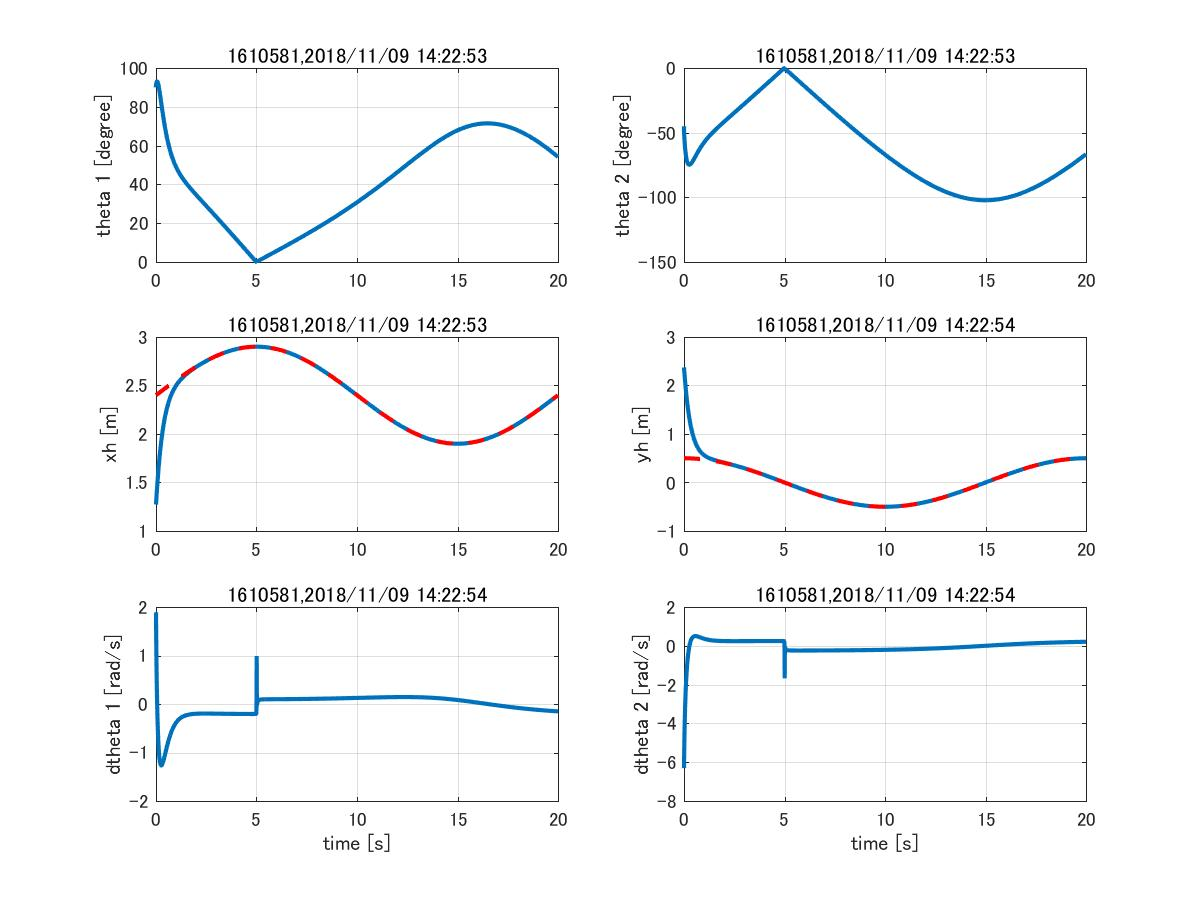
\includegraphics[width=7cm]{../img/kadai45/jpg_hand_zihen_auto_zikan_2.jpg}
            \caption{時変2のときの数値シミュレーションにおける応答時間.}
          \end{center}
        \end{figure}
        %%%%%%%%%%%%%%%%%%%%%%%%%%%%%%%%%%%%%%%%%%%%%%%%%%%%%%%%%%%%%%%%%%%%%%%%%%%%%%%%%
        \begin{figure}[H]
          % 図12
          \begin{center}
            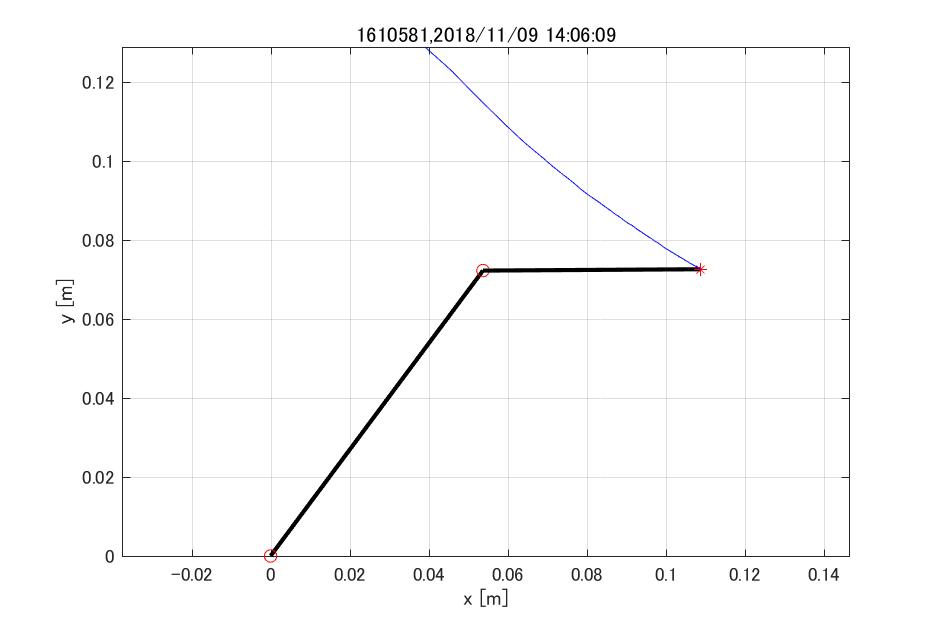
\includegraphics[width=7cm]{../img/kadai45/jpg_zissai_hand_zifuhen_saisyu_sise.jpg}
            \caption{時不変のときの実機実験における最終姿勢.}
          \end{center}
        \end{figure}
        
        \begin{figure}[H]
          % 図12
          \begin{center}
            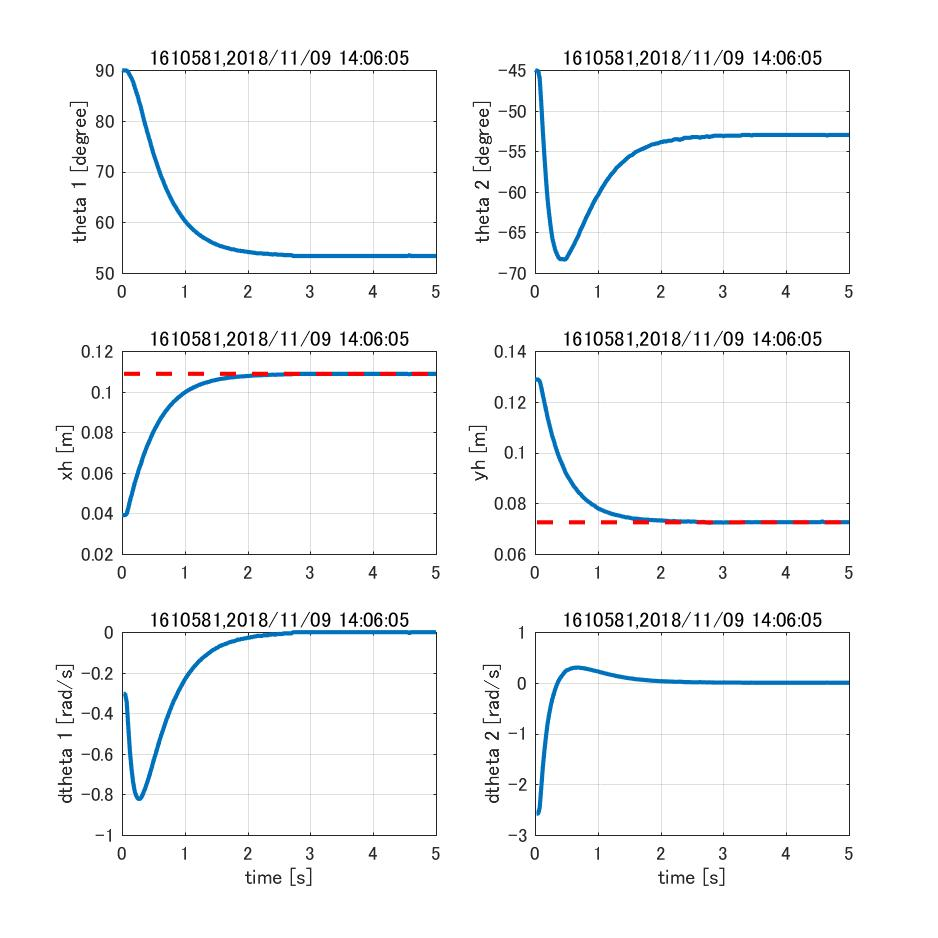
\includegraphics[width=7cm]{../img/kadai45/jpg_zissai_hand_zifuhen_auto_zikan.jpg}
            \caption{時不変のときの実機実験における応答時間.}
          \end{center}
        \end{figure}
        %%%%%%%%%%%%%%%%%%%%%%%%%%%%%%%%%%%%%%%%%%%%%%%%%%%%%%%%%%%%%%%%%%%%%%%%%%%%%%%%%
        \begin{figure}[H]
          % 図12
          \begin{center}
            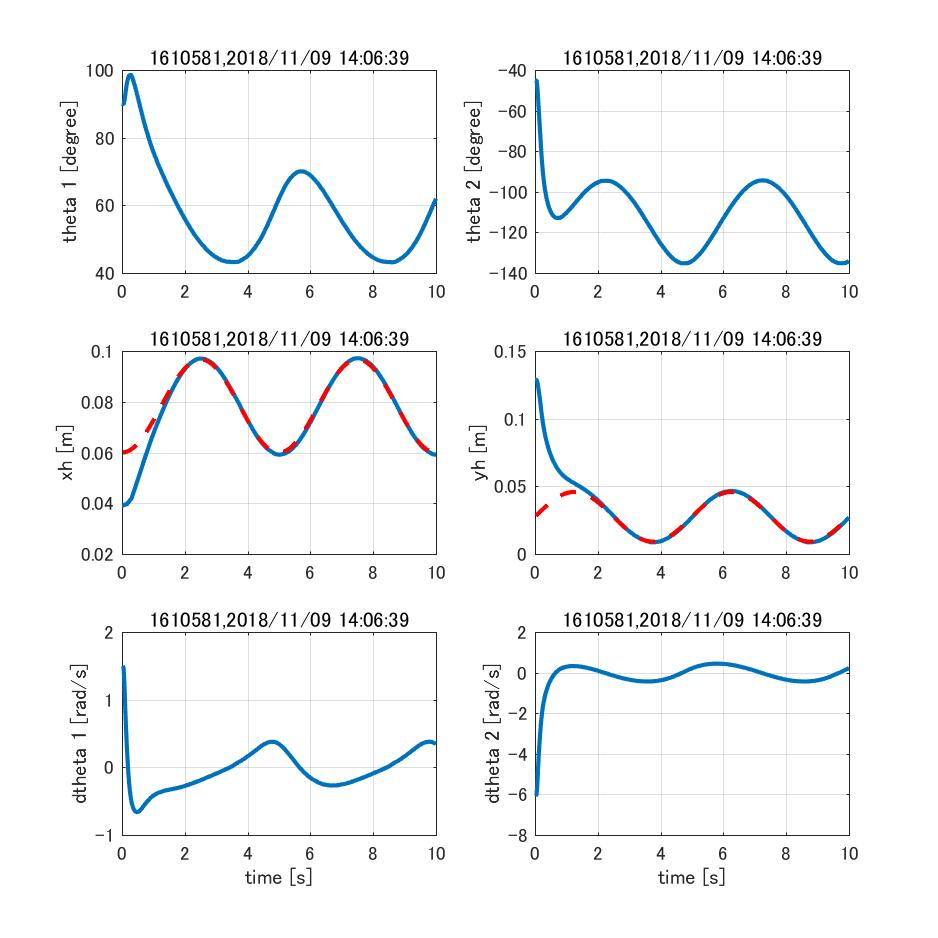
\includegraphics[width=7cm]{../img/kadai45/jpg_zissai_hand_zihen_saisyu_sise_1.jpg}
            \caption{時変1のときの実機実験における最終姿勢.}
          \end{center}
        \end{figure}
        
        \begin{figure}[H]
          % 図12
          \begin{center}
            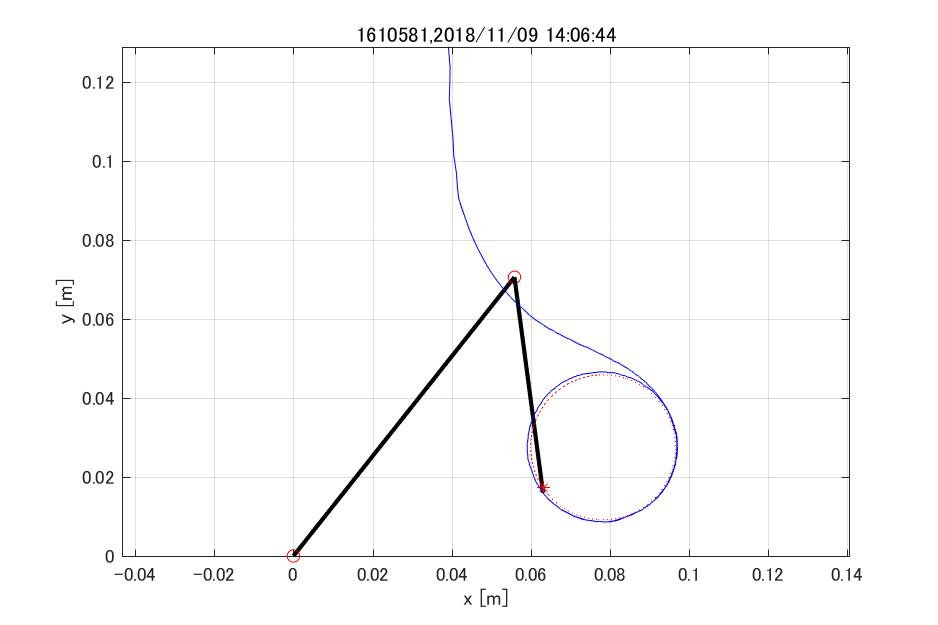
\includegraphics[width=7cm]{../img/kadai45/jpg_zissai_hand_zihen_auto_zikan_1.jpg}
            \caption{時変1のときの実機実験における応答時間.}
          \end{center}
        \end{figure}
        %%%%%%%%%%%%%%%%%%%%%%%%%%%%%%%%%%%%%%%%%%%%%%%%%%%%%%%%%%%%%%%%%%%%%%%%%%%%%%%%%
        \begin{figure}[H]
          % 図12
          \begin{center}
            \includegraphics[width=7cm]{../img/kadai45/jpg_zissai_hand_zihen_saisyu_sise_1.jpg}
            \caption{時変2のときの実機実験における最終姿勢.}
          \end{center}
        \end{figure}
        
        \begin{figure}[H]
          % 図12
          \begin{center}
            \includegraphics[width=7cm]{../img/kadai45/jpg_zissai_hand_zihen_auto_zikan_1.jpg}
            \caption{時変2のときの実機実験における応答時間.}
          \end{center}
        \end{figure}
        %%%%%%%%%%%%%%%%%%%%%%%%%%%%%%%%%%%%%%%%%%%%%%%%%%%%%%%%%%%%%%%%%%%%%%%%%%%%%%%%%
        \begin{figure}[H]
          % 図12
          \begin{center}
            \includegraphics[width=7cm]{../img/kadai45/jpg_game_pad_hand_zihen_saisyu_sise.jpg}
            \caption{ゲームパッドで操作したときの姿勢.}
          \end{center}
        \end{figure}
        
        \begin{figure}[H]
          % 図12
          \begin{center}
            \includegraphics[width=7cm]{../img/kadai45/game_outo.jpg}
            \caption{ゲームパッドで操作した時の応答時間.}
          \end{center}
        \end{figure}
    \end{enumerate}
  
  \subsection{レポート課題}
    \begin{enumerate}
      \item 課題A.
        ロボット制御における特異点とは,一直線上にロボットアームが並んだときに逆運動学計算の解が得られず,制御できなくなる点を表す. また,特異姿勢とは,[4]より,マニュピレータの
        姿勢によってはヤコビ行列が退化し逆行列が存在しなくなることがある. このような姿勢を特異姿勢と呼ぶ.
        これらの現象を回避するためには,[4]では可操作性楕円体の体積は手先の動かしやすさを表していると考えられており,ロボットの特異点回避に利用できると述べられている.
      \item 課題B.
    \end{enumerate}

  \subsection{感想}
    実際にロボットを動かすのはとても楽しかった. 


% 結果
\begin{thebibliography}{3}
\bibitem{bunken2}岡島 寛, 西村悠樹, 松永信智. モデル誤差抑制補償に基づく非線形システムのフィードバック線形化. 計測自動制御学会論文集(2014).
\bibitem{bunken2}安川電機. ロボットゼミナール第4回最終回. 安川電機ホームページ(2012).
\bibitem{bunken2}大隈 久. ロボットの基礎. \bibitem{bunken2}安川電機. ロボットゼミナール第4回最終回. 精密工学会誌 Vol.73 No.10, 2007.
\bibitem{bunken2}田中 正史. 仮想空間におけるロボットの軌道教示・生成システムの開発. 奈良先端科学技術大学院大学 修士論文(2002).
\bibitem{bunken2}電気通信大学 知能機械工学基礎実験テキスト p32~37.

\end{thebibliography}
\end{document}